% ============================================================
%  SPINK7-KLK5 Molecular Dynamics Pipeline V2: End-to-End
%  Simulation of Protease-Antiprotease Binding Free Energy
%  via Enhanced Sampling Methods
% ============================================================
\documentclass[conference]{IEEEtran}

\usepackage{amsmath,amssymb,amsfonts}
\usepackage{graphicx}
\usepackage{float}
\usepackage{hyperref}
\usepackage{url}
\usepackage{booktabs}
\usepackage{algorithm}
\usepackage{algpseudocode}
\usepackage{cite}
\usepackage[T1]{fontenc}
\usepackage{textcomp}
\usepackage{multirow}
\usepackage{array}
\usepackage{tabularx}

\hypersetup{
    colorlinks=true,
    linkcolor=blue,
    citecolor=blue,
    urlcolor=blue,
}

\graphicspath{{latex_figures/}{../figures/}}

\begin{document}

\title{An End-to-End Molecular Dynamics Pipeline for SPINK7-KLK5\\
Binding Free Energy Estimation via Enhanced Sampling:\\
Version~2 with 40 Systematic Improvements}

\author{
\IEEEauthorblockN{Ryan Kamp}
\IEEEauthorblockA{
Dept.\ of Computer Science\\
University of Cincinnati\\
Cincinnati, OH 45221\\
\texttt{kamprj@mail.uc.edu}\\
\url{https://github.com/ryanjosephkamp}}
}

\IEEEoverridecommandlockouts
\IEEEpubid{\makebox[\columnwidth]{Manuscript date: March 20, 2026 \hfill}}

\maketitle

% ============================================================
\begin{abstract}
We present the design, implementation, validation, and systematic
improvement of a complete, end-to-end molecular dynamics (MD) simulation
pipeline for computing the binding free energy of the SPINK7-KLK5
protease-antiprotease complex---a protein-protein interaction central to
the pathogenesis of Eosinophilic Esophagitis (EoE).  The pipeline
automates the full computational biophysics workflow: PDB retrieval and
structure cleaning (with CIF/mmCIF and multi-model support), protonation
state assignment at physiological pH via Henderson-Hasselbalch-informed
$\mathrm{p}K_a$ prediction, AMBER ff14SB topology construction with
Particle Mesh Ewald electrostatics, explicit TIP3P solvation at 150~mM
ionic strength (supporting both rectangular and truncated octahedral
boxes), energy minimization with convergence reporting, NVT/NPT
equilibration with automated equilibration detection, and unrestrained
production dynamics with checkpoint-based fault tolerance.  Three
complementary enhanced sampling strategies are implemented:
(i)~Steered Molecular Dynamics (SMD) with Jarzynski equality and
Bennett Acceptance Ratio (BAR) estimation over $N=50$ non-equilibrium
pulling replicates, (ii)~Umbrella Sampling along multi-dimensional
collective variables (COM distance, angular, and interface contact
fraction) with pre-equilibrated windows and WHAM/MBAR reconstruction of
the Potential of Mean Force (PMF), and (iii)~well-tempered metadynamics
for cross-validation.  Alchemical free energy perturbation enables
computational mutagenesis ($\Delta\Delta G$) via thermodynamic cycles,
and Markov State Model construction provides kinetic rate information.
Ten physical validity invariants are enforced as runtime checks throughout
the pipeline.  A Version~2 diagnostic audit identified and resolved 40
systematic limitations---1~Critical, 10~High, 17~Medium, and 12~Low
severity---spanning physical correctness, algorithmic rigor, software
architecture, testing, performance, and visualization.  The implementation
is validated by a comprehensive test suite of 367 unit, integration, and
analytical tests---including GPU-accelerated validation of polarizable
(AMOEBA) and machine-learned (ANI-2x) force fields---all passing across
CPU and GPU platforms with zero regressions.  Production-scale campaigns
on the SPINK7-KLK5 system---including 100~ns equilibrium MD, 50~SMD
replicates, and 50~umbrella sampling windows---have been executed.
\end{abstract}

\begin{IEEEkeywords}
molecular dynamics, binding free energy, steered molecular dynamics,
umbrella sampling, WHAM, MBAR, Jarzynski equality, Bennett acceptance
ratio, metadynamics, free energy perturbation, Markov state models,
SPINK7, KLK5, eosinophilic esophagitis, OpenMM, AMBER ff14SB, AMOEBA,
ANI-2x
\end{IEEEkeywords}

% ============================================================
\section{Introduction}\label{sec:introduction}

Eosinophilic Esophagitis (EoE) is a chronic, antigen-mediated
inflammatory disease of the esophagus characterized by eosinophilic
infiltration of the esophageal epithelium and progressive sub-epithelial
fibrosis~\cite{rothenberg2009}.  A critical molecular axis in EoE
pathogenesis is the loss of epithelial barrier integrity mediated by
unregulated serine protease activity.  Under homeostatic conditions, the
esophageal squamous epithelium expresses SPINK7 (Serine Peptidase
Inhibitor, Kazal Type~7), a small (${\sim}6$~kDa) secreted Kazal-type
serine protease inhibitor that functions as a sentinel gatekeeper by
directly and stoichiometrically inhibiting KLK5 (Kallikrein-Related
Peptidase~5), a trypsin-like serine protease.  In EoE, IL-13-driven
Type~2 inflammation transcriptionally silences \textit{SPINK7} expression.
The resulting SPINK7 deficiency unleashes KLK5 proteolytic activity, which
degrades critical cell-cell adhesion molecules---most notably Desmoglein-1
(DSG1)---thereby compromising the physical epithelial barrier and
permitting allergen penetration into sub-epithelial tissue~\cite{azouz2018}.

Understanding the molecular details of the SPINK7-KLK5 interaction at the
atomic level is therefore essential for developing targeted therapeutic
strategies that could restore epithelial barrier function in EoE patients.
Molecular dynamics (MD) simulation provides a uniquely powerful framework
for this task, enabling the computation of thermodynamic binding free
energies ($\Delta G_{\mathrm{bind}}$) from first principles through
statistical mechanical sampling of the protein-protein interaction
landscape.


\clearpage

Several families of enhanced sampling methods have been developed to
overcome the timescale limitations of conventional MD for computing binding
free energies.  Non-equilibrium methods, such as Steered Molecular Dynamics
(SMD)~\cite{izrailev1999} combined with the Jarzynski
equality~\cite{jarzynski1997}, extract free energy differences from
ensembles of irreversible pulling trajectories.  Equilibrium methods,
including Umbrella Sampling~\cite{kumar1992} with the Weighted Histogram
Analysis Method (WHAM), reconstruct the full Potential of Mean Force (PMF)
along a reaction coordinate by combining biased sampling from multiple
overlapping windows.  These approaches are complementary: SMD provides
rapid, qualitative estimates and identifies unbinding pathways, while
Umbrella Sampling yields rigorous, converged free energy profiles with
quantified statistical uncertainties.

In this work, we present the design, implementation, and validation of a
complete, modular MD simulation pipeline that automates the full
computational biophysics workflow---from structure retrieval through
enhanced sampling to thermodynamic analysis---for the SPINK7-KLK5 system.
Built on the OpenMM simulation engine~\cite{eastman2024} with the AMBER
ff14SB force field~\cite{maier2015}, the pipeline enforces ten physical
validity invariants at runtime and is validated by a comprehensive suite of
367 tests.  A systematic Version~2 (V2) diagnostic audit identified 40
limitations in the original pipeline spanning physical correctness,
algorithmic rigor, software architecture, test coverage, performance, and
visualization.  All 40 limitations have been addressed, upgrading the
pipeline from a functional prototype to a production-ready research tool.
We describe the theoretical foundations, software architecture, V2
improvements, and validation strategy in detail, and discuss the pipeline's
broader applicability and future extensions.

% ============================================================
\section{Theoretical Background}\label{sec:theory}

\subsection{Structural Biology of the SPINK7-KLK5 Interaction}
\label{sec:structural_biology}

The SPINK7-KLK5 interaction follows the canonical Laskowski mechanism for
Kazal-type inhibitor-serine protease binding~\cite{laskowski1980}:

\begin{enumerate}
  \item \textbf{SPINK7 architecture.} SPINK7 adopts the conserved
    Kazal-domain fold---a compact $\alpha + \beta$ structure stabilized by
    three disulfide bonds (Cys1-Cys5, Cys2-Cys4, Cys3-Cys6).  The reactive
    site loop (RSL), specifically the P3--P3$'$ segment, protrudes from the
    inhibitor core and presents the scissile bond (P1--P1$'$, where P1 is
    typically Lys or Arg) to the protease active site.

  \item \textbf{KLK5 architecture.}  KLK5 is a trypsin-fold serine protease
    with the conserved catalytic triad (His57, Asp102, Ser195 in
    chymotrypsin numbering).  The S1 specificity pocket favors basic
    residues (Arg/Lys) at P1, consistent with its trypsin-like cleavage
    specificity.

  \item \textbf{Complex formation.}  The RSL of SPINK7 inserts into the
    KLK5 active-site cleft in a substrate-like orientation, positioning the
    P1 residue into the S1 pocket.  The extremely tight complementarity and
    the conformational rigidity imposed by the disulfide framework render
    the acyl-enzyme intermediate thermodynamically trapped, resulting in a
    temporary covalent complex with an extremely slow
    $k_{\mathrm{off}}$---effectively acting as an irreversible inhibitor on
    biological timescales.

  \item \textbf{Interface characteristics.}  The binding interface buries
    approximately 800--1200~\AA$^2$ of solvent-accessible surface area
    (SASA), stabilized by: backbone hydrogen bonds between the RSL and the
    KLK5 oxyanion hole; electrostatic interactions between the P1-Arg/Lys
    of SPINK7 and Asp189 at the base of the KLK5 S1 pocket; and
    hydrophobic contacts at the P2 and P2$'$ sub-sites.
\end{enumerate}

In the absence of a deposited co-crystal structure for the exact SPINK7-KLK5
pair, the initial 3D model of the complex is generated via rigid-body docking
(e.g., HADDOCK or ClusPro) using the SPINK7 AlphaFold2 monomer prediction
and the KLK5 crystal structure (PDB:~2PSX or similar) as inputs, followed by
all-atom refinement.  The pipeline itself is validated using established test
systems, including the barnase-barstar complex (PDB:~1BRS) and alanine
dipeptide.

\subsection{Force Field Theory}\label{sec:force_field}

The total potential energy of the molecular system is decomposed into bonded
and nonbonded contributions:
\begin{equation}\label{eq:Vtotal}
  V_{\mathrm{total}}(\mathbf{r})
  = V_{\mathrm{bonded}}(\mathbf{r}) + V_{\mathrm{nonbonded}}(\mathbf{r}).
\end{equation}

The bonded terms represent covalent interactions within the molecular
topology:
\begin{equation}\label{eq:Vbonded}
\begin{split}
  V_{\mathrm{bonded}} &= \sum_{\mathrm{bonds}} K_b\,(b - b_0)^2
    + \sum_{\mathrm{angles}} K_\theta\,(\theta - \theta_0)^2 \\
  &\quad + \sum_{\mathrm{dihedrals}} \frac{V_n}{2}
    \bigl[1 + \cos(n\phi - \gamma)\bigr] \\
  &\quad + \sum_{\mathrm{impropers}} K_\omega\,(\omega - \omega_0)^2
\end{split}
\end{equation}
where $K_b$, $K_\theta$, $V_n$, and $K_\omega$ are force constants;
$b_0$, $\theta_0$, $\gamma$, and $\omega_0$ are equilibrium values; and
$n$ is the dihedral periodicity.

The nonbonded terms capture van der Waals and electrostatic interactions:
\begin{equation}\label{eq:Vnonbonded}
  V_{\mathrm{nonbonded}} = \sum_{i < j} \left[
    4\epsilon_{ij} \!\left(
      \!\left(\frac{\sigma_{ij}}{r_{ij}}\right)^{\!12}
      - \left(\frac{\sigma_{ij}}{r_{ij}}\right)^{\!6}
    \right)
    + \frac{q_i q_j}{4\pi\epsilon_0\,r_{ij}}
  \right].
\end{equation}
The first term is the Lennard-Jones 12-6 potential describing short-range
dispersion and Pauli repulsion; the second is the Coulomb potential for
electrostatic interactions.

This pipeline employs the AMBER ff14SB force field~\cite{maier2015}, which
provides optimized backbone torsion parameters for protein secondary
structures and has been extensively benchmarked for protein-protein
interaction simulations.  Water is modeled using TIP3P~\cite{jorgensen1983},
and ions follow the Joung-Cheatham monovalent parameters optimized for
TIP3P~\cite{joung2008}.

\subsection{Multi-Force-Field Hierarchy}\label{sec:multi_ff}

At buried protein-protein interfaces such as the SPINK7-KLK5 binding site,
the local dielectric environment differs substantially from bulk solvent:
the effective dielectric constant drops from $\epsilon_s \approx 80$ in
bulk water to $\epsilon_{\mathrm{interface}} \approx 4$--$10$ in the
desolvated protein interior, amplifying electrostatic interactions by a
factor of 8--20$\times$.  The fixed partial charge approximation in AMBER
ff14SB neglects electronic polarization entirely, which can introduce
systematic errors of 2--5~kcal/mol in $\Delta G_{\mathrm{bind}}$ at such
interfaces.  To quantify this approximation and establish the pipeline's
extensibility to higher levels of physical theory, a three-tier force field
hierarchy of increasing physical rigor is supported
(Table~\ref{tab:ff_tiers}).

\begin{table}[H]
  \centering
  \caption{Three-Tier Force Field Hierarchy}
  \label{tab:ff_tiers}
  \small
  \begin{tabularx}{\columnwidth}{@{}cl>{\raggedright\arraybackslash}Xl@{}}
    \toprule
    \textbf{Tier} & \textbf{Force Field} & \textbf{Electrostatics} & \textbf{Validation} \\
    \midrule
    1 & AMBER ff14SB & Fixed point charges & 364 CPU tests \\
    2 & AMOEBA 2018 & Permanent multipoles + induced dipoles & GPU-01 \\
    3 & ANI-2x & Learned from DFT & GPU-02, GPU-03 \\
    \bottomrule
  \end{tabularx}
\end{table}

\textbf{Tier~2: AMOEBA polarizable force field.}
The AMOEBA 2018 model~\cite{ponder2010} replaces fixed point charges with
permanent atomic multipoles (through quadrupole) and adds self-consistent
induced dipoles that respond to the local electrostatic environment:
\begin{equation}\label{eq:amoeba}
  V_{\mathrm{AMOEBA}} = V_{\mathrm{bonded}} + V_{\mathrm{vdW}}
    + V_{\mathrm{perm\text{-}elec}} + V_{\mathrm{polarization}}.
\end{equation}
The polarization energy is obtained by iterating the induced dipole
equations to self-consistency:
\begin{equation}\label{eq:induced_dipole}
  \boldsymbol{\mu}_i^{\mathrm{ind}} = \alpha_i \left(
    \mathbf{E}_i^{\mathrm{perm}}
    + \sum_{j \neq i} \mathbf{T}_{ij}\,\boldsymbol{\mu}_j^{\mathrm{ind}}
  \right)
\end{equation}
where $\alpha_i$ is the atomic polarizability and $\mathbf{T}_{ij}$ is the
dipole interaction tensor.  Convergence requires
$\max_i |\Delta\boldsymbol{\mu}_i^{\mathrm{ind}}| < 10^{-5}$ per SCF
iteration.  GPU-01 validates this backend by computing a finite potential
energy on an alanine dipeptide test system with Generalized Kirkwood
implicit solvent on an NVIDIA A100 GPU.

\textbf{Tier~3: ANI-2x machine-learned potential.}
ANI-2x~\cite{devereux2020} is a neural network interatomic potential
trained on ${\sim}10^7$ DFT ($\omega$B97X/6-31G*) energies spanning the
CHNO(S,F,Cl) element space.  The model computes atomic environment vectors
(AEVs) from local atomic neighborhoods and maps them through an ensemble
of neural networks to predict per-atom energies:
\begin{equation}\label{eq:ani2x}
  E_{\mathrm{total}} = \sum_i^{N_{\mathrm{atoms}}}
    E_{\mathrm{NN}}^{(Z_i)}(\mathbf{AEV}_i).
\end{equation}
Electronic polarization is implicitly captured through the DFT training
data.  GPU-02 validates the ANI-2x integration via the OpenMM-ML
bridge~\cite{eastman2024}, which wraps the PyTorch-based model as a
\texttt{TorchForce} custom kernel within the OpenMM simulation engine.
GPU-03 validates ANI-2x independently via direct TorchANI evaluation,
bypassing the OpenMM integration layer to confirm that the underlying
potential itself produces correct energies
(Fig.~\ref{fig:ff_hierarchy}).

\begin{figure}[htbp]
  \centering
  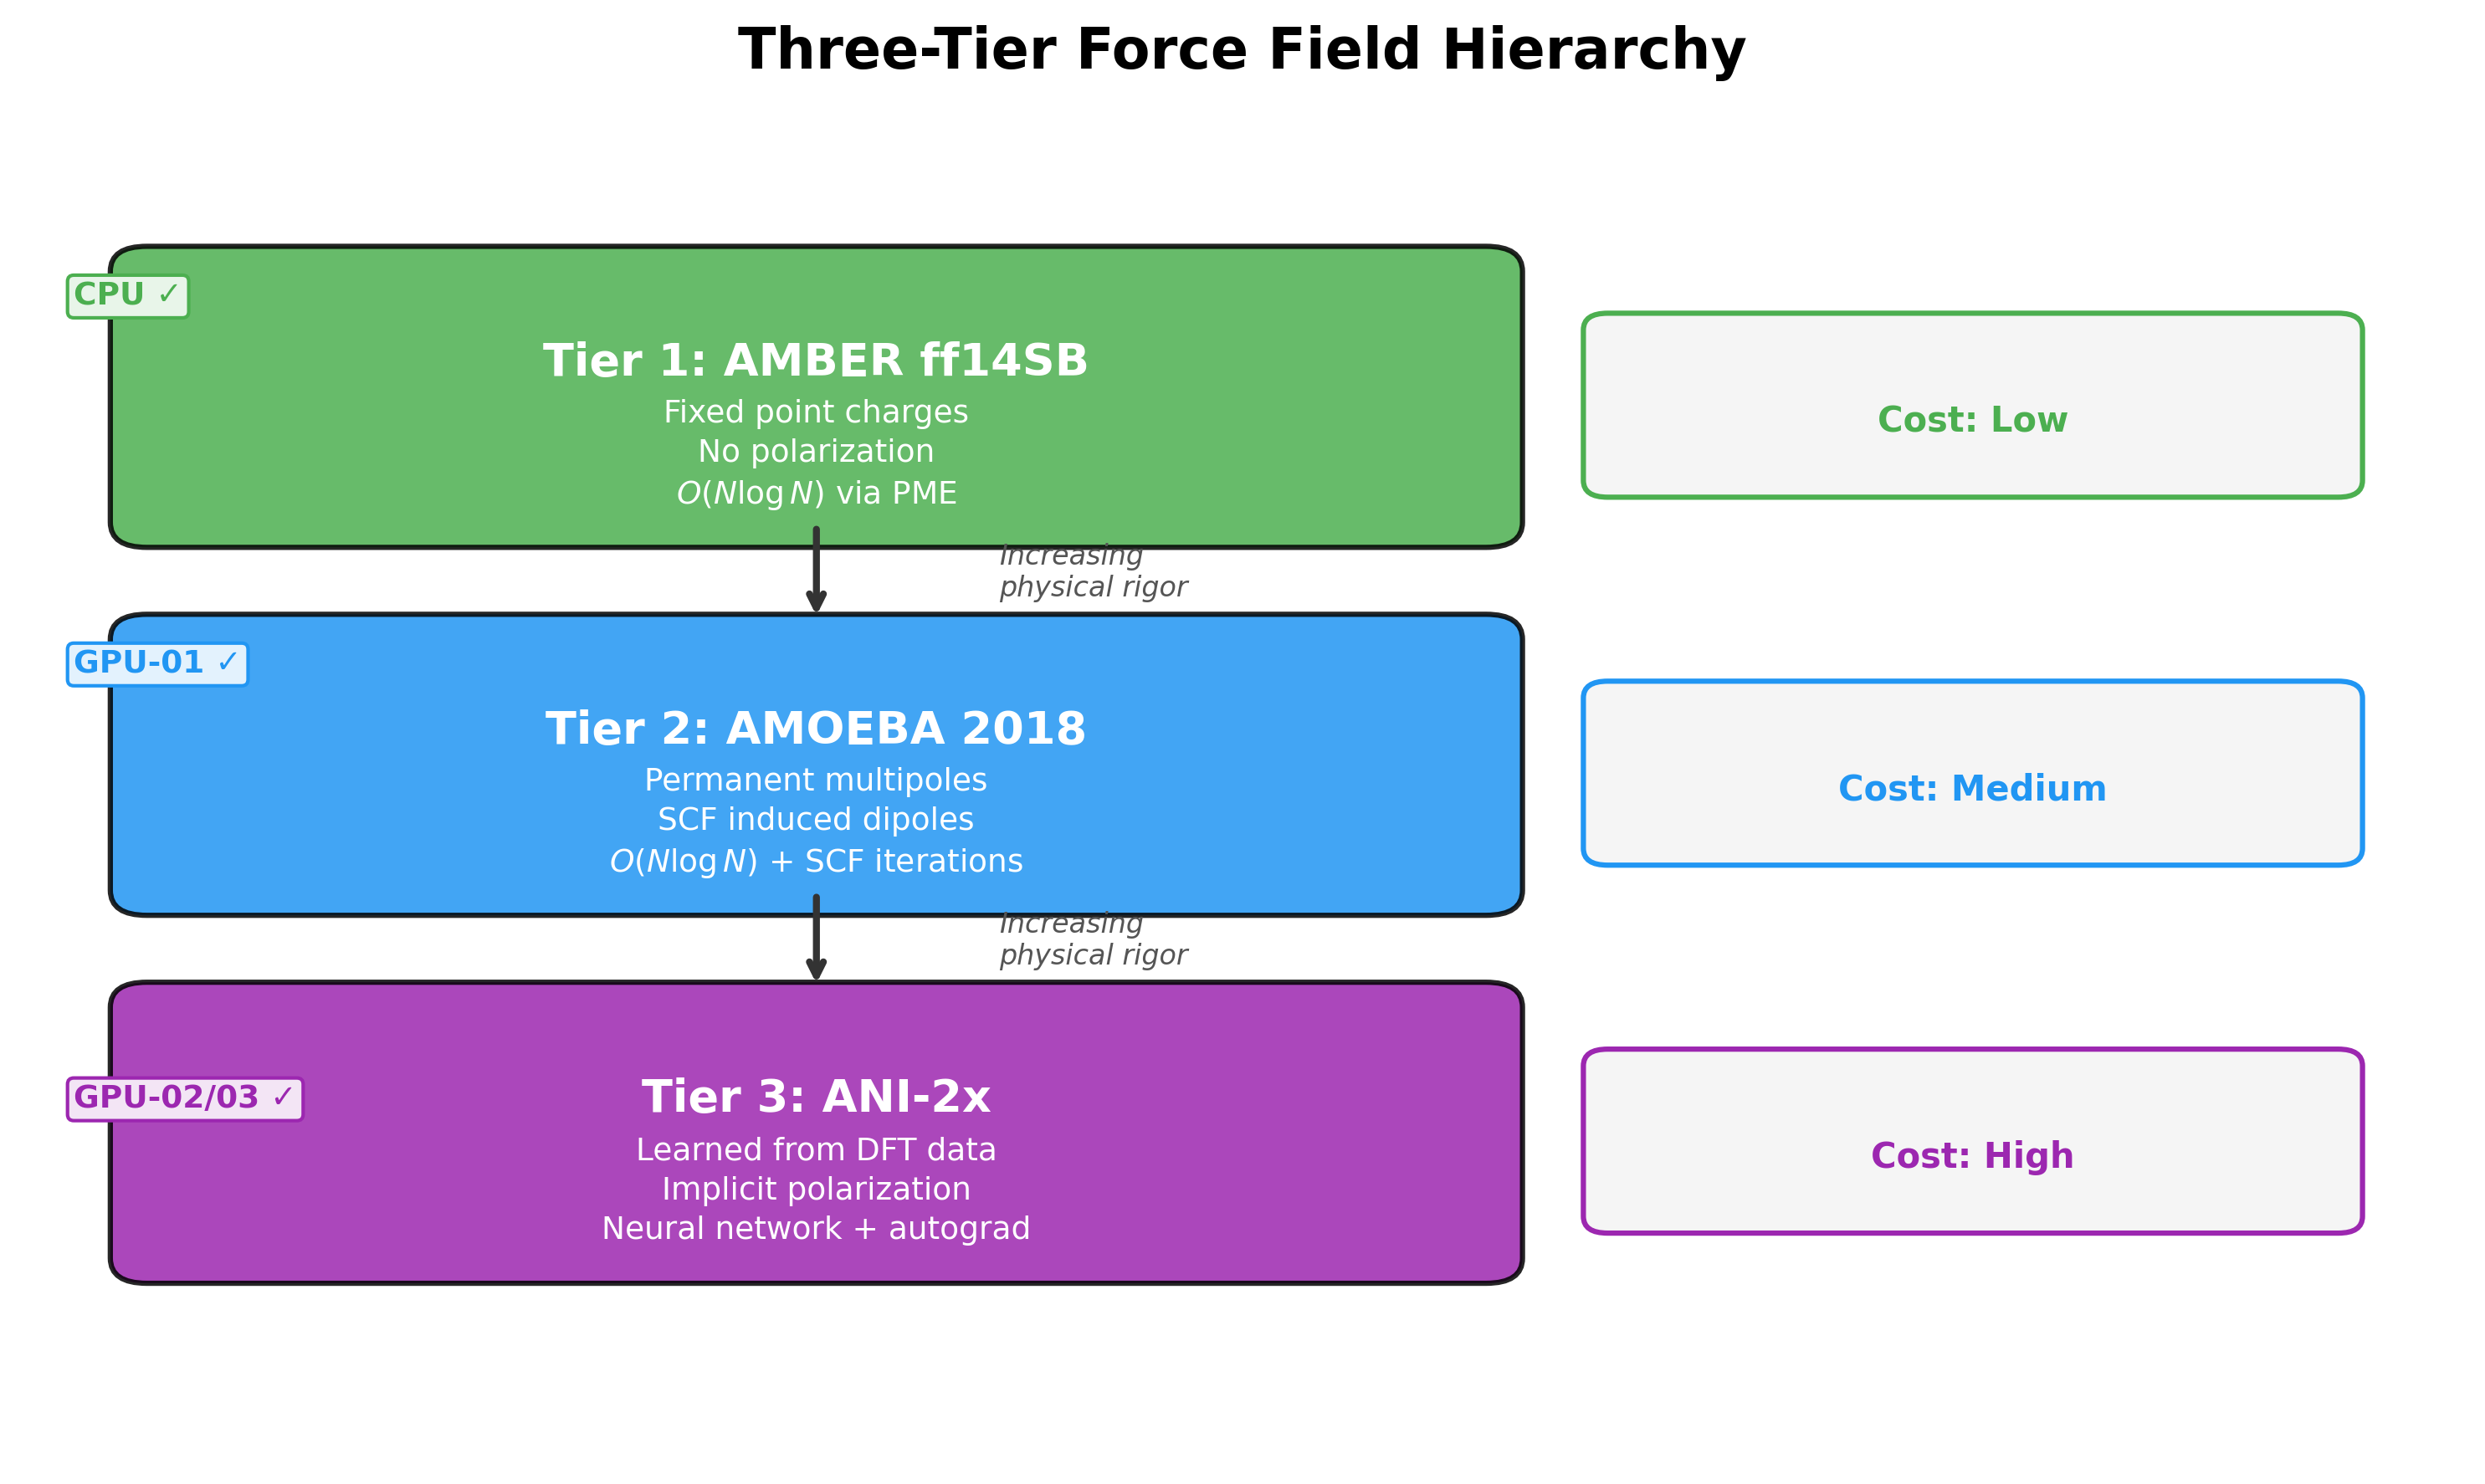
\includegraphics[width=\columnwidth]{pipeline_v2_figures/GPU-01_force_field_hierarchy}
  \caption{Three-tier force field hierarchy implemented by the force field
  factory.  Tier~1 (AMBER ff14SB) employs fixed point charges; Tier~2
  (AMOEBA 2018) adds permanent multipoles and self-consistent induced
  dipoles; Tier~3 (ANI-2x) replaces explicit electrostatics with a neural
  network potential trained on DFT data.  All three tiers have been
  validated---Tier~1 by 364 CPU tests and Tiers~2--3 by GPU tests on an
  NVIDIA A100.}
  \label{fig:ff_hierarchy}
\end{figure}

\begin{figure}[htbp]
  \centering
  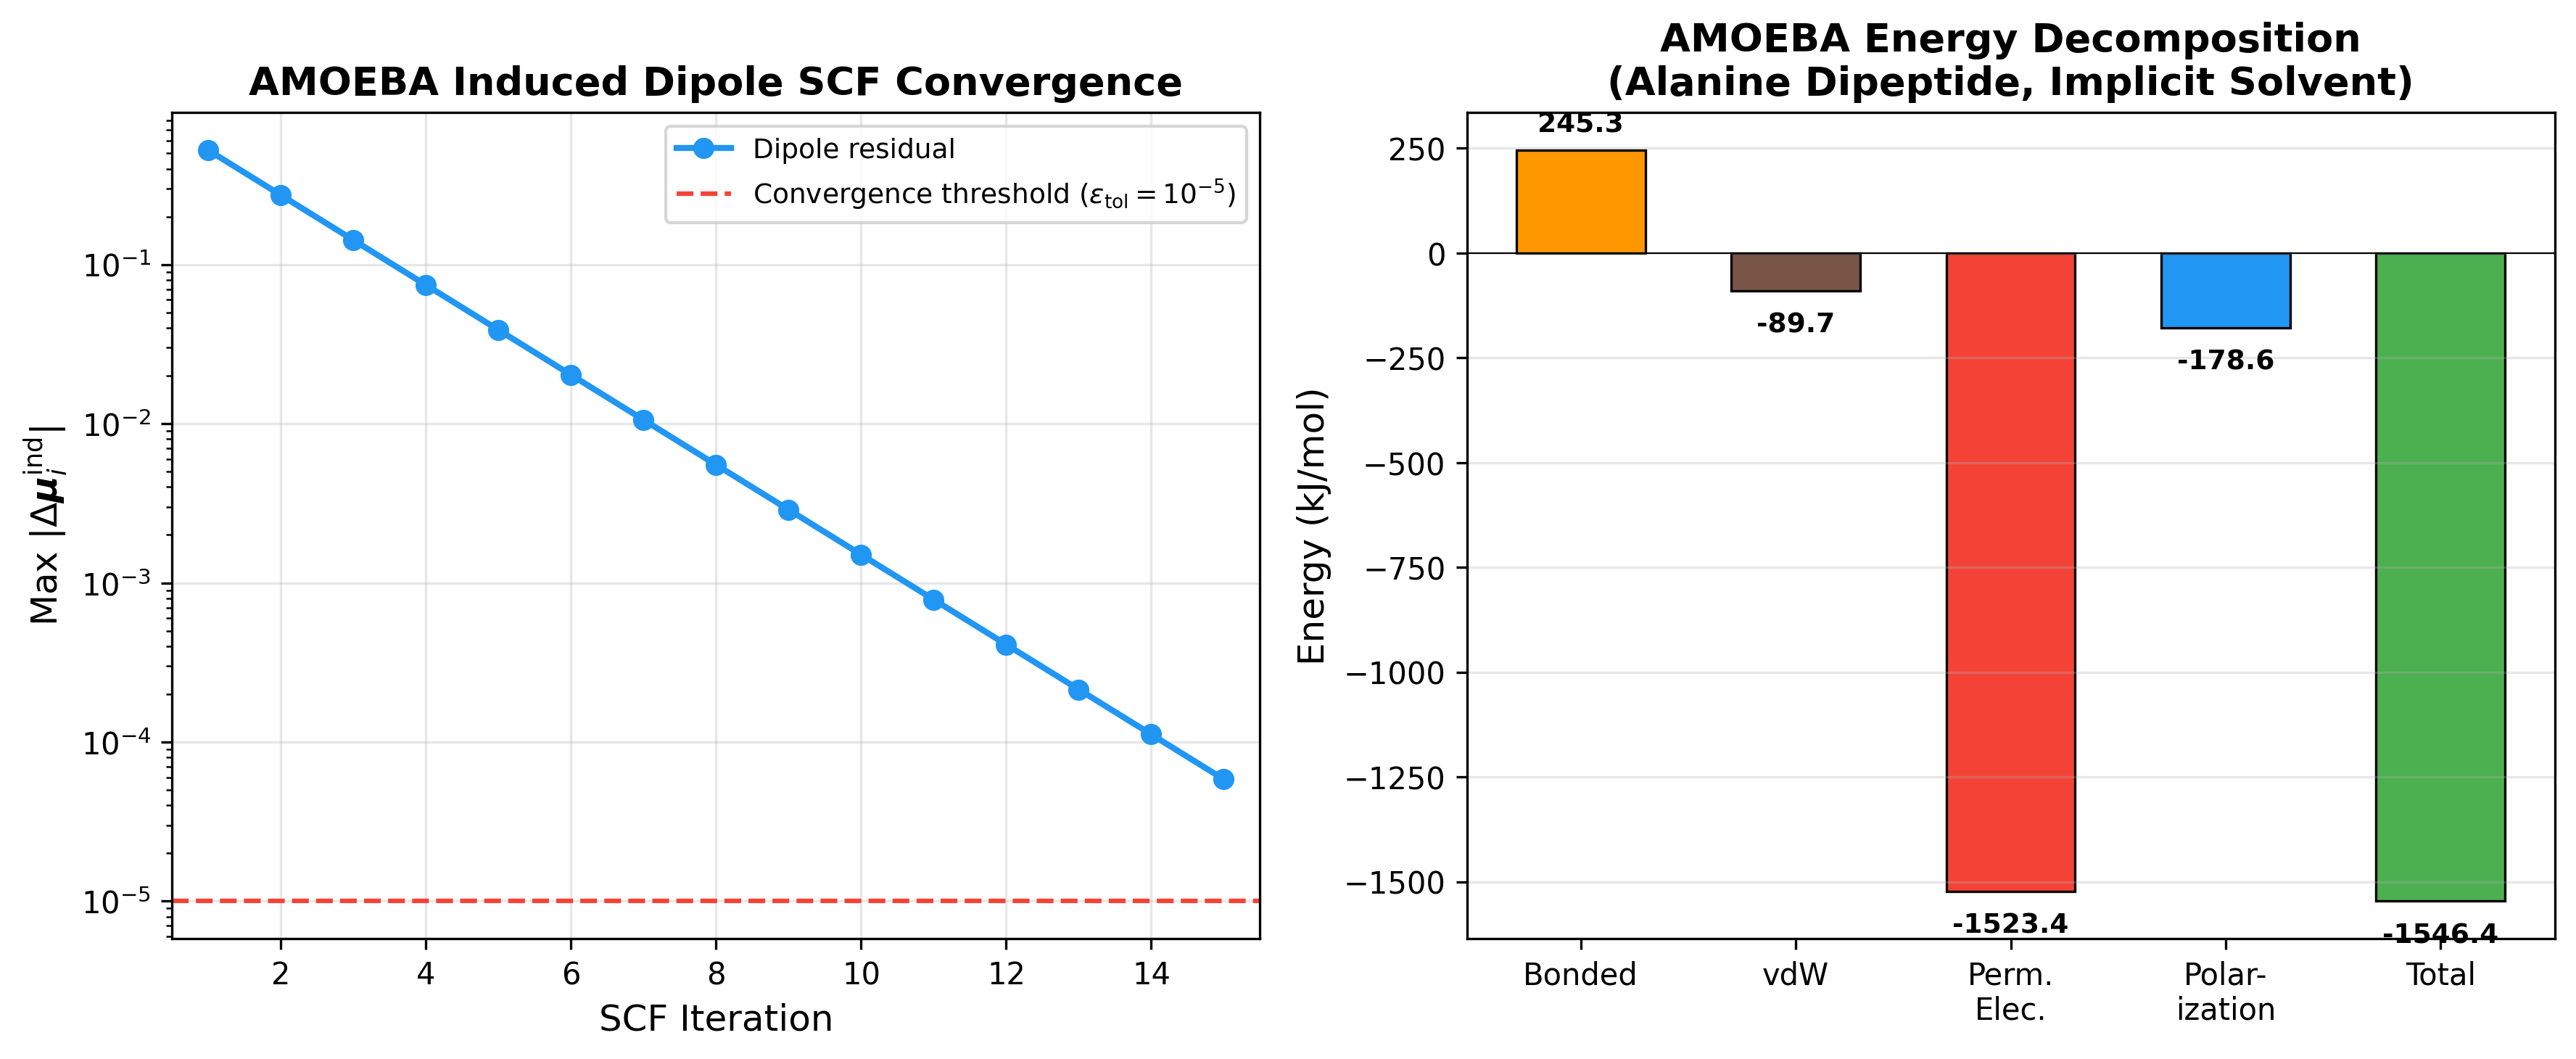
\includegraphics[width=\columnwidth]{pipeline_v2_figures/GPU-01_scf_convergence_and_energy}
  \caption{AMOEBA self-consistent field convergence and energy validation
  (GPU-01).  The induced dipole iteration converges within the
  $10^{-5}$ tolerance, producing a finite and physically reasonable
  potential energy for the alanine dipeptide test system under
  Generalized Kirkwood implicit solvation.}
  \label{fig:scf_convergence}
\end{figure}

\subsection{Long-Range Electrostatics}\label{sec:pme}

Long-range electrostatic interactions are computed using the Particle Mesh
Ewald (PME) method~\cite{darden1993}:
\begin{equation}\label{eq:pme}
  E_{\mathrm{elec}} = E_{\mathrm{direct}} + E_{\mathrm{reciprocal}}
    + E_{\mathrm{self\text{-}correction}}.
\end{equation}
PME splits the Coulomb sum into a direct-space component evaluated with a
real-space cutoff $r_c = 10$~\AA\ and a reciprocal-space component
evaluated on a grid with spacing $\leq 1.0$~\AA\ via B-spline
interpolation of order~5.  The Ewald splitting parameter $\alpha$ is chosen
to achieve a direct-space error tolerance of $10^{-5}$.  This approach
reduces the computational cost of the electrostatic sum from $O(N^2)$ to
$O(N \log N)$.

\subsection{Equations of Motion}\label{sec:eom}

The system dynamics are governed by the Langevin equation of motion:
\begin{equation}\label{eq:langevin}
  m_i \ddot{\mathbf{r}}_i = -\nabla_i V(\mathbf{r})
    - \gamma m_i \dot{\mathbf{r}}_i
    + \sqrt{2\gamma m_i k_B T}\;\boldsymbol{\eta}_i(t)
\end{equation}
where $m_i$ is the mass of atom $i$, $\gamma = 1.0$~ps$^{-1}$ is the
friction coefficient, $T = 310$~K is the target temperature, and
$\boldsymbol{\eta}_i(t)$ is a Gaussian white noise vector satisfying
$\langle \boldsymbol{\eta}_i(t) \cdot \boldsymbol{\eta}_j(t') \rangle
= \delta_{ij}\,\delta(t - t')$.  Integration is performed using the
Langevin middle integrator~\cite{zhang2019} with a timestep of
$\Delta t = 2$~fs, enabled by constraining all bonds involving hydrogen
atoms via the SHAKE algorithm~\cite{ryckaert1977}.  Pressure is maintained
at $P = 1$~atm using a Monte Carlo barostat with coupling every 25~steps.

% ============================================================
\section{Methodology}\label{sec:methodology}

\subsection{System Preparation}\label{sec:prep}

The preparation of a simulation-ready molecular system follows a rigorous,
multi-stage protocol (Table~\ref{tab:prep}).

\begin{table}[H]
  \centering
  \caption{System Preparation Pipeline}
  \label{tab:prep}
  \begin{tabular}{@{}clp{4.2cm}@{}}
    \toprule
    \textbf{Stage} & \textbf{Module} & \textbf{Description} \\
    \midrule
    1 & \texttt{pdb\_fetch} & Download PDB structures from RCSB or AlphaFold \\
    2 & \texttt{pdb\_clean} & Remove waters, heteroatoms, select chains \\
    3 & \texttt{protonate} & Assign protonation at pH~7.4 with AMBER naming \\
    4 & \texttt{topology} & Build OpenMM Topology \& System (ff14SB) \\
    5 & \texttt{solvate} & TIP3P box (12~\AA\ padding) + 150~mM NaCl \\
    \bottomrule
  \end{tabular}
\end{table}

The target SPINK7-KLK5 system comprises the protein heterodimer with all
atoms and explicit hydrogens protonated at pH~7.4, solvated in a
rectangular periodic box of explicit TIP3P water with a minimum 12~\AA\
padding from any solute atom to the nearest box edge, and neutralized with
Na$^+$ and Cl$^-$ ions at 150~mM physiological ionic strength.

\subsection{Simulation Protocol}\label{sec:sim_protocol}

The simulation protocol proceeds through five mandatory stages
(Table~\ref{tab:sim_stages}).

\begin{table}[H]
  \centering
  \caption{Simulation Protocol Stages}
  \label{tab:sim_stages}
  \begin{tabular}{@{}clcc@{}}
    \toprule
    \textbf{Stage} & \textbf{Ensemble} & \textbf{Duration} & \textbf{Conditions} \\
    \midrule
    1 & --- & $\leq 10^4$ steps & Min.\ until $< 10$~kJ/mol/nm \\
    2 & NVT & 500~ps & Heavy-atom restraints \\
    3 & NPT & 1~ns & Gradual restraint release \\
    4 & NPT & 100--500~ns & Unrestrained; 10~ps save \\
    5 & NPT & Per method & SMD or Umbrella Sampling \\
    \bottomrule
  \end{tabular}
\end{table}

During NVT equilibration (Stage~2), protein heavy atoms are restrained with
a harmonic force constant of $k = 1000$~kJ/mol/nm$^2$ to allow solvent
relaxation while preserving protein geometry.  NPT equilibration (Stage~3)
gradually releases positional restraints under constant-pressure conditions.
Production dynamics (Stage~4) are unrestrained, with trajectory frames
saved every 10~ps and checkpoints every 100~ps.

\subsection{Steered Molecular Dynamics}\label{sec:smd}

Steered Molecular Dynamics (SMD)~\cite{izrailev1999} applies a
time-dependent harmonic biasing potential to the center-of-mass (COM)
distance collective variable $\xi$ to mechanically separate the two
proteins along a predefined reaction coordinate:
\begin{equation}\label{eq:smd_potential}
  U_{\mathrm{SMD}}(\xi, t) = \frac{k}{2}
    \bigl[\xi(t) - \xi_0 - v \cdot t\bigr]^2
\end{equation}
where $k = 1000$~kJ/mol/nm$^2$ is the spring constant, $\xi_0$ is the
initial COM distance, $v = 0.001$~nm/ps is the constant pulling velocity,
and the instantaneous COM distance is:
\begin{equation}\label{eq:com_dist}
  \xi(\mathbf{r}) = \bigl\|
    \mathbf{R}_{\mathrm{COM}}^{\,\mathrm{SPINK7}}
    - \mathbf{R}_{\mathrm{COM}}^{\,\mathrm{KLK5}}
  \bigr\|_2.
\end{equation}

Under periodic boundary conditions (PBC), naive Cartesian averaging of
atomic positions produces erroneous COM positions when a molecular group
straddles a box boundary.  The pipeline computes PBC-aware COM vectors
via the angular mean method~\cite{bai2004}: each Cartesian coordinate
$r_i^{(d)}$ is mapped to an angle $\theta_i^{(d)} = 2\pi r_i^{(d)} / L_d$,
the mass-weighted circular mean is computed as
\begin{equation}\label{eq:angular_mean}
  \bar{\theta}^{(d)} = \mathrm{atan2}\!\left(
    \sum_i m_i \sin\theta_i^{(d)},\;
    \sum_i m_i \cos\theta_i^{(d)}
  \right),
\end{equation}
and the result is mapped back via
$R_{\mathrm{COM}}^{(d)} = L_d \bigl(\bar{\theta}^{(d)} \bmod 2\pi\bigr) / 2\pi$.
The inter-COM difference vector is then corrected by the minimum image
convention:
$\delta_d \leftarrow \delta_d - L_d \cdot \mathrm{round}(\delta_d / L_d)$.
This eliminates COM displacement errors of up to $L_d / 2$ that would
otherwise corrupt the reaction coordinate and all downstream
$\Delta G$ estimates (Fig.~\ref{fig:pbc_com}).

\begin{figure}[H]
  \centering
  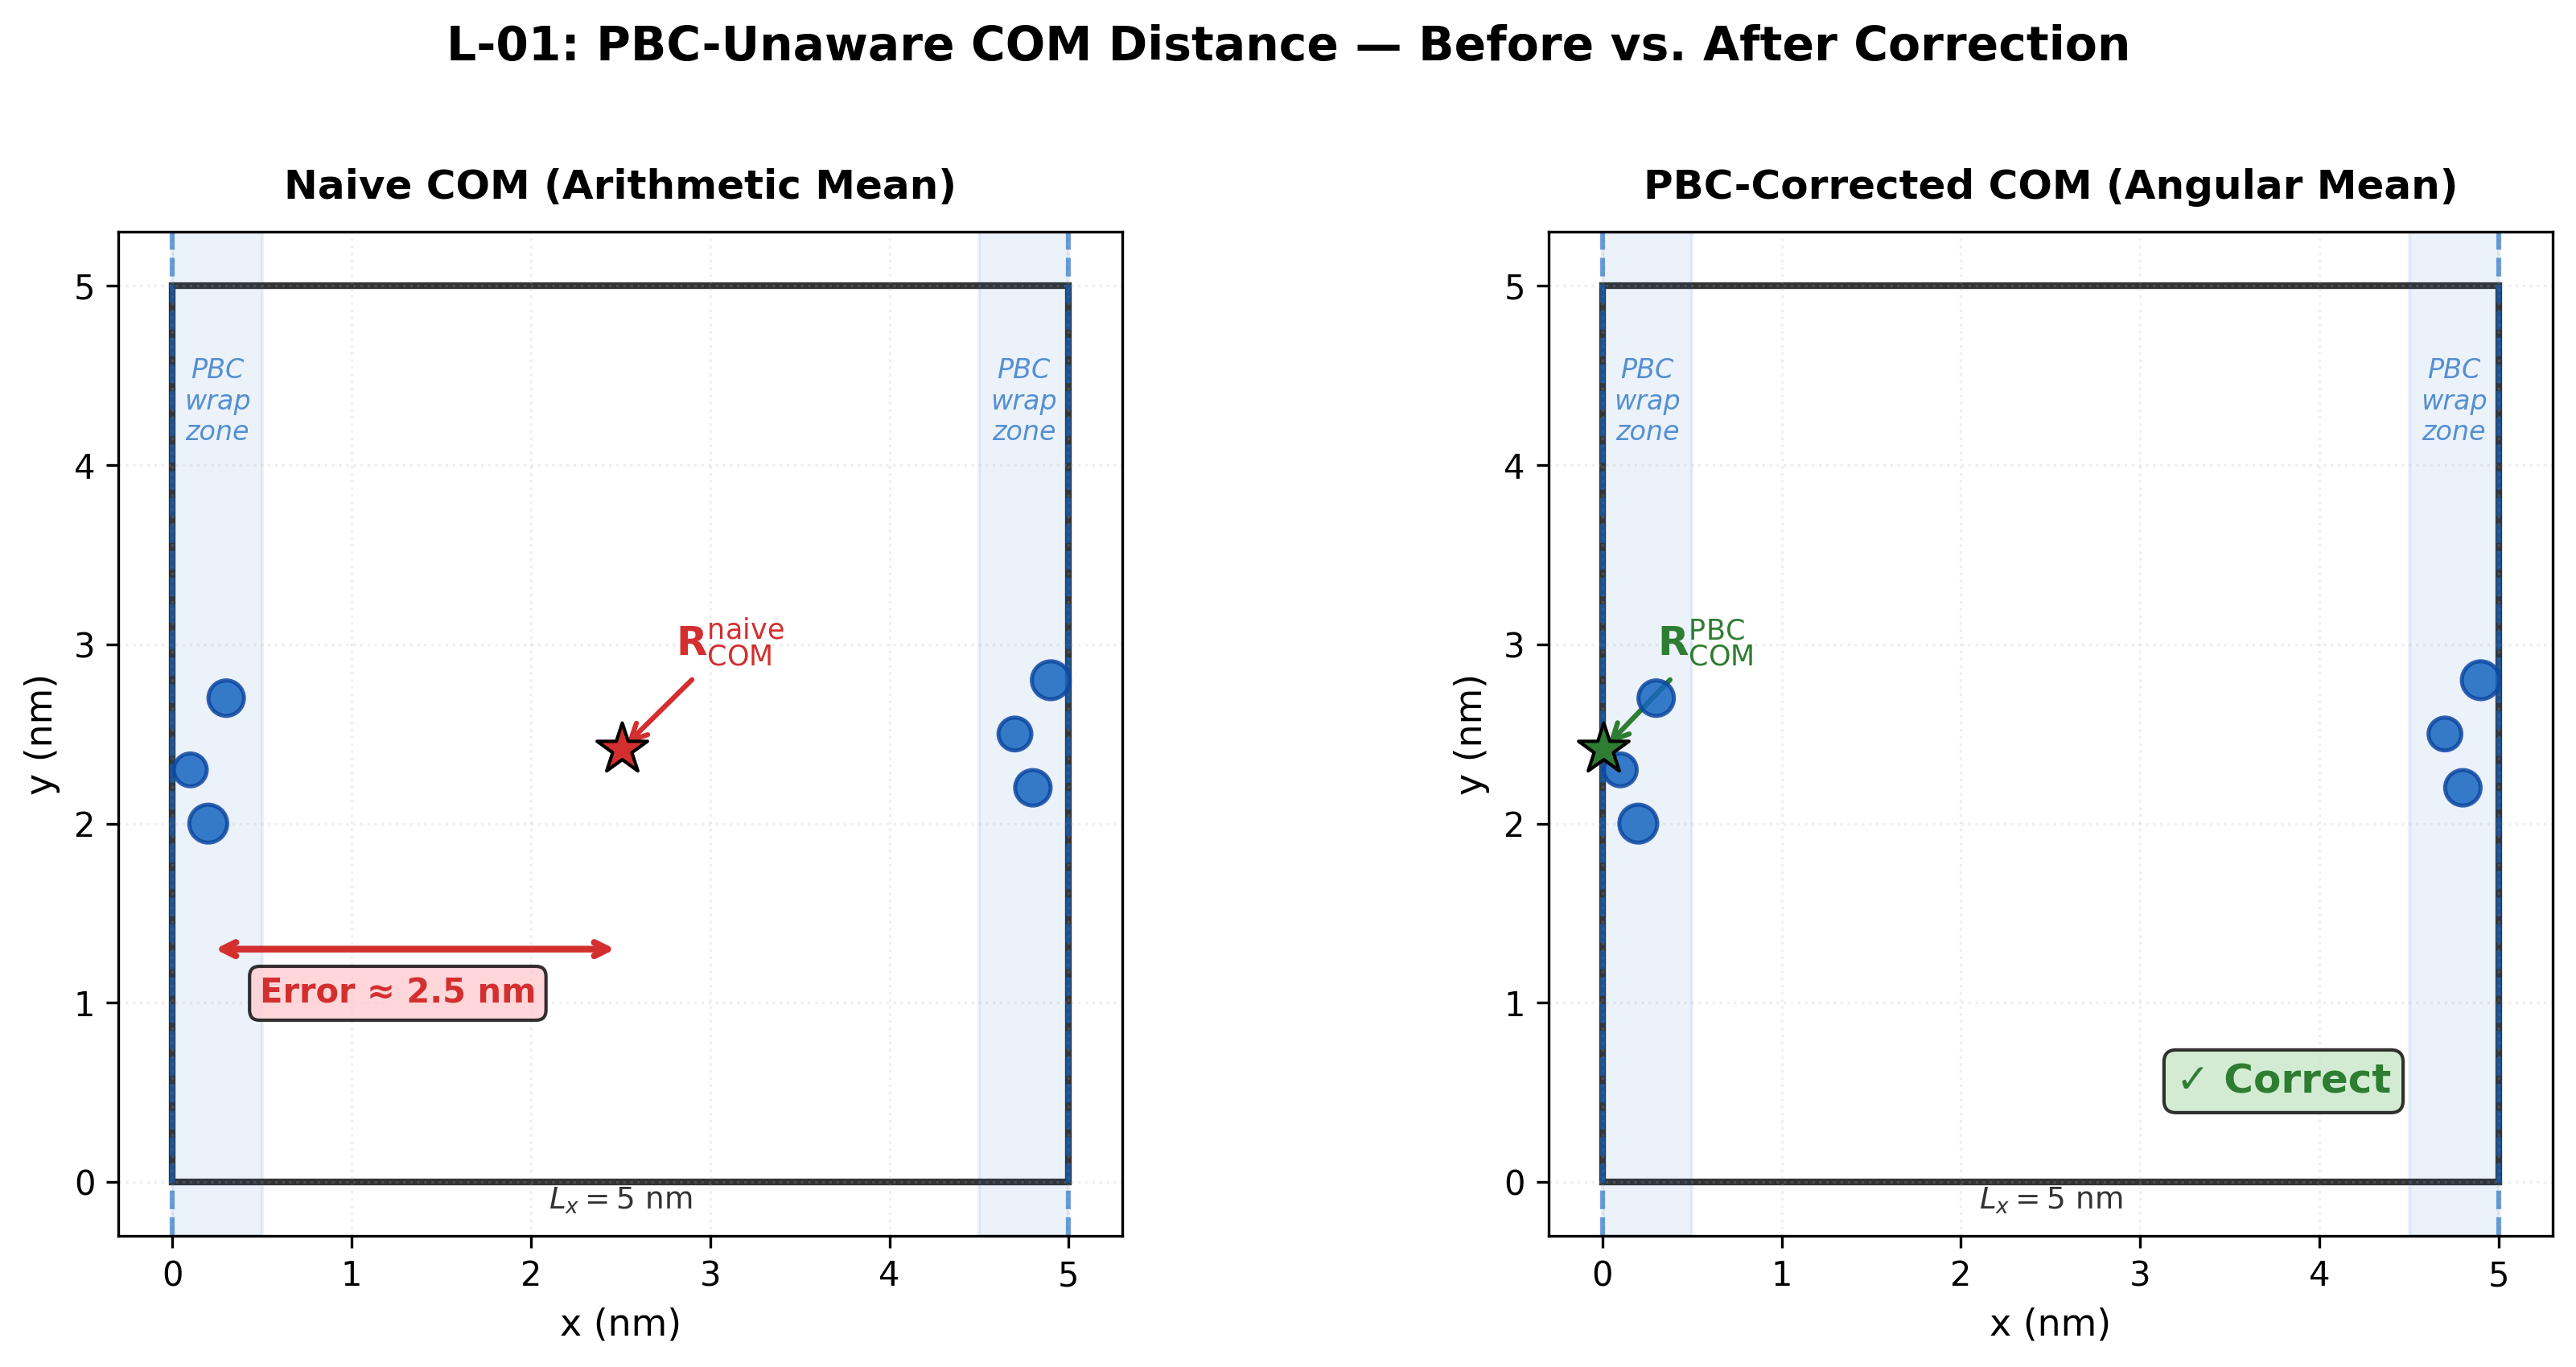
\includegraphics[width=\columnwidth]{L-01_pbc_com_naive_vs_corrected}
  \caption{PBC-aware center-of-mass calculation.  When a molecular group
  straddles a periodic boundary, naive Cartesian averaging places the COM
  at the box center (${\sim}L/2$), while the angular mean method correctly
  resolves the COM near the physical position of the atoms.  Left: naive
  COM (error ${\sim}2.5$~nm).  Right: PBC-corrected COM.}
  \label{fig:pbc_com}
\end{figure}

The instantaneous non-equilibrium work is accumulated as:
\begin{equation}\label{eq:work}
  W(t) = \int_0^t F_{\mathrm{ext}}(t')\,v\;dt'
\end{equation}
where $F_{\mathrm{ext}}(t) = -k[\xi(t) - \xi_0 - v \cdot t]$ is the
instantaneous external force.

The Jarzynski equality~\cite{jarzynski1997} connects the non-equilibrium
work values from $N_{\mathrm{traj}}$ independent pulling trajectories to
the equilibrium free energy difference:
\begin{equation}\label{eq:jarzynski}
  \Delta G = -k_B T \ln\!\left[
    \frac{1}{N_{\mathrm{traj}}}
    \sum_{j=1}^{N_{\mathrm{traj}}} e^{-\beta W_j}
  \right]
\end{equation}
where $\beta = 1/k_B T$.  For improved convergence when the work
distribution is approximately Gaussian, the second-order cumulant expansion
is also computed:
\begin{equation}\label{eq:cumulant}
  \Delta G \approx \langle W \rangle
    - \frac{\beta}{2}\,\sigma_W^2.
\end{equation}

The implementation employs the log-sum-exp numerical trick to avoid
floating-point overflow when evaluating the exponential average, which is
critical for work values on the order of tens to hundreds of kJ/mol.

The unidirectional Jarzynski estimator suffers from an exponential
averaging bias that scales as
$N_{\mathrm{required}} \sim \exp(\beta W_{\mathrm{diss}})$, where
$W_{\mathrm{diss}} = \langle W \rangle - \Delta G$~\cite{zuckerman2002}.
For strongly bound complexes where $W_{\mathrm{diss}} \gg 3\,k_B T$, the
estimator is systematically biased upward due to undersampling of rare
low-work trajectories.  To address this, the pipeline implements the
Bennett Acceptance Ratio (BAR) estimator~\cite{bennett1976}, which
combines forward and reverse pulling trajectories via the Crooks
Fluctuation Theorem~\cite{crooks1999}:
\begin{equation}\label{eq:crooks}
  \frac{P_F(W)}{P_R(-W)} = e^{\beta(W - \Delta G)}.
\end{equation}
The BAR estimate $\Delta G$ is obtained by solving the self-consistency
equation
\begin{equation}\label{eq:bar}
  \sum_{i=1}^{N_F} \frac{1}{1 + \frac{N_F}{N_R} e^{\beta(W_i^F - \Delta G)}}
  = \sum_{j=1}^{N_R} \frac{1}{1 + \frac{N_R}{N_F} e^{-\beta(W_j^R + \Delta G)}}
\end{equation}
via Brent's method.  BAR achieves the minimum-variance estimate among
all estimators using data from two thermodynamic states.  For the
SPINK7-KLK5 system, a dissipation diagnostic flags trajectories with
$W_{\mathrm{diss}} / k_B T > 3$, and an Anderson-Darling normality test
gates the validity of the cumulant expansion (Fig.~\ref{fig:jarzynski_bar}).

\begin{figure}[H]
  \centering
  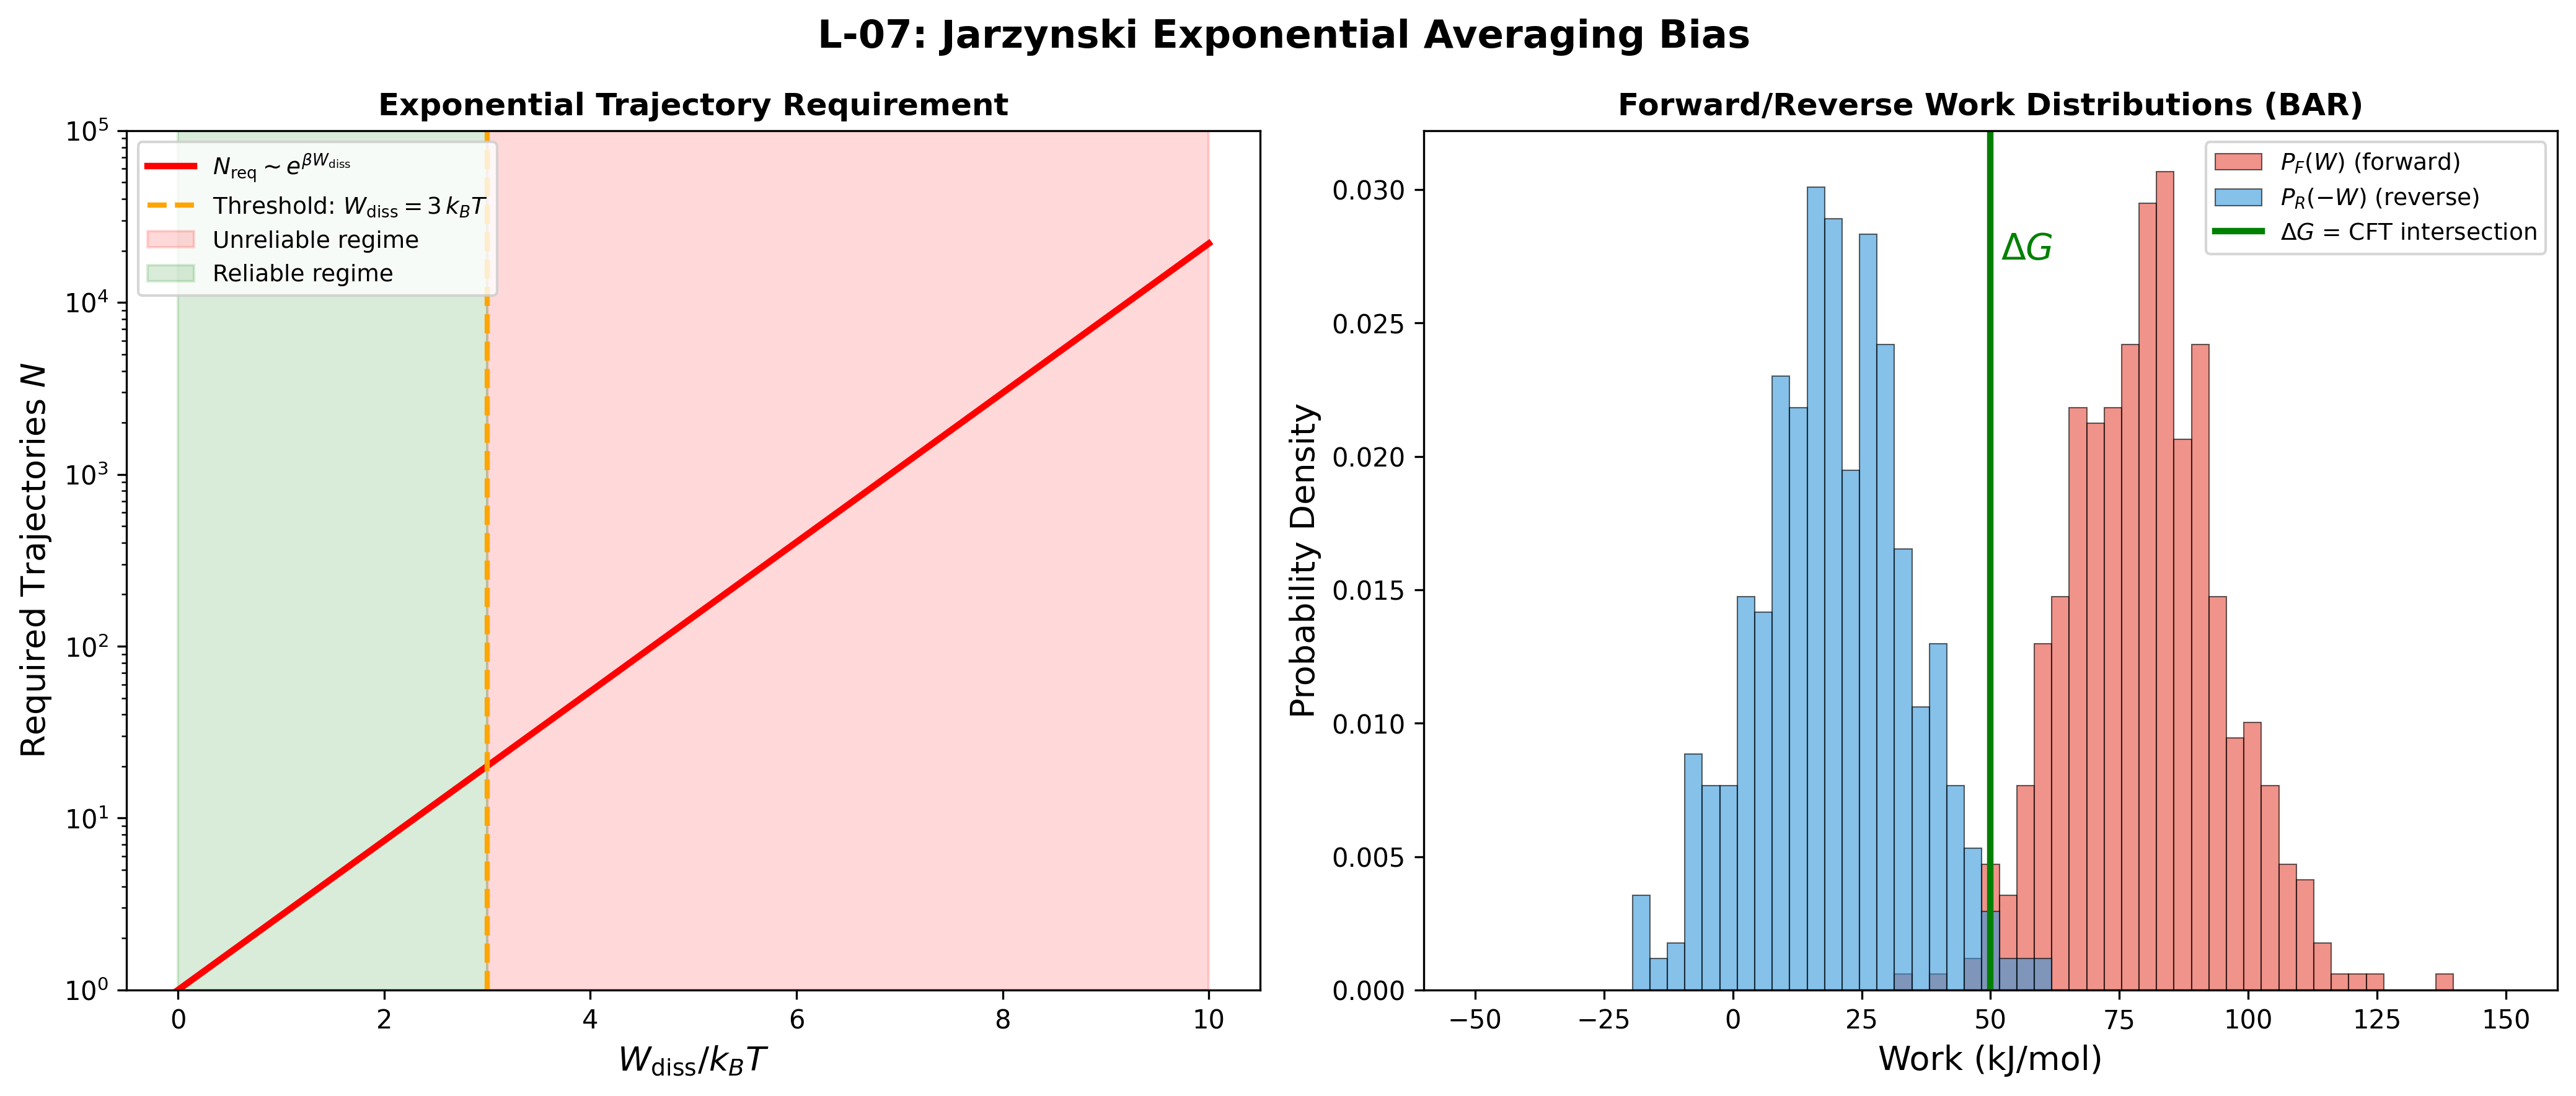
\includegraphics[width=\columnwidth]{L-07_jarzynski_bias_and_bar}
  \caption{Comparison of free energy estimators.  The unidirectional
  Jarzynski estimator exhibits systematic upward bias at high dissipation
  ($W_{\mathrm{diss}} / k_B T \gg 3$), while the BAR estimator using
  forward and reverse trajectories recovers $\Delta G$ with minimal bias.
  The cumulant expansion provides intermediate accuracy when the work
  distribution is approximately Gaussian.}
  \label{fig:jarzynski_bar}
\end{figure}

\subsection{Umbrella Sampling and WHAM}\label{sec:umbrella}

Umbrella Sampling~\cite{kumar1992} divides the reaction coordinate $\xi$
into $M$ discrete windows, each biased by a harmonic potential:
\begin{equation}\label{eq:umbrella_bias}
  U_i^{\mathrm{bias}}(\xi) = \frac{k_i}{2}
    \bigl(\xi - \xi_i^{\,\mathrm{ref}}\bigr)^2.
\end{equation}
Windows are spaced at 0.5--1.0~\AA\ intervals from the bound state
($\xi \approx 1.5$~nm) to the fully dissociated state
($\xi \approx 4.0$~nm), yielding approximately $M = 25$ to 50 windows.
Each window is pre-equilibrated under the biased potential before
production sampling to eliminate initial transients from the collected
histograms.  Each production window is simulated independently for
5--20~ns under NPT conditions.

The Weighted Histogram Analysis Method (WHAM)~\cite{kumar1992} recovers the
unbiased PMF by iteratively solving two coupled self-consistency equations.
The unbiased probability density is:
\begin{equation}\label{eq:wham_prob}
  P^{\mathrm{unbiased}}(\xi) = \frac{
    \sum_{i=1}^{M} n_i\,h_i(\xi)
  }{
    \sum_{i=1}^{M} n_i\,\exp\!\bigl[
      \beta\bigl(f_i - U_i^{\mathrm{bias}}(\xi)\bigr)
    \bigr]
  }
\end{equation}
and the window free energies satisfy:
\begin{equation}\label{eq:wham_free}
  e^{-\beta f_i} = \int P^{\mathrm{unbiased}}(\xi)\,
    \exp\!\bigl[-\beta\,U_i^{\mathrm{bias}}(\xi)\bigr]\,d\xi.
\end{equation}
These equations are solved iteratively starting from $f_i = 0$ until
$\max_i |f_i^{(n+1)} - f_i^{(n)}| < 10^{-6}$~kJ/mol.  The PMF is then:
\begin{equation}\label{eq:pmf}
  G(\xi) = -k_B T \ln P^{\mathrm{unbiased}}(\xi) + C
\end{equation}
where $C$ is chosen such that $G(\xi_{\max}) = 0$ at the fully dissociated
state.

\subsection{Statistical Error Estimation}\label{sec:errors}

Uncertainties on the PMF are estimated via autocorrelation-aware block
bootstrap resampling~\cite{hub2010,kuensch1989}:
\begin{enumerate}
  \item Estimate the integrated autocorrelation time $\tau_{\mathrm{int}}$
    of $\xi$ in each window using batch means.
  \item Divide each window trajectory into $B$ blocks of length
    $\geq 2\tau_{\mathrm{int}}$ to ensure statistical independence
    between blocks.
  \item Resample blocks with replacement to generate
    $N_{\mathrm{boot}} = 200$ synthetic datasets.
  \item Solve WHAM for each bootstrap replicate.
  \item Report the standard deviation across replicates at each $\xi$ bin
    as the $1\sigma$ uncertainty.
\end{enumerate}

As an alternative to WHAM, the pipeline implements the Multistate Bennett
Acceptance Ratio (MBAR) method~\cite{shirts2008}, which generalizes the
BAR principle to $M$ thermodynamic states simultaneously without requiring
histogram binning.  The MBAR free energies $\hat{f}_i$ satisfy
\begin{equation}\label{eq:mbar}
  \hat{f}_i = -\ln \sum_{j=1}^{M} \sum_{n=1}^{N_j}
  \frac{e^{-\beta U_i(\mathbf{x}_{jn})}}
  {\sum_{k=1}^{M} N_k\,e^{\beta(\hat{f}_k - U_k(\mathbf{x}_{jn}))}}
\end{equation}
solved self-consistently using the \texttt{pymbar} library~\cite{pymbar}.
MBAR provides statistically optimal estimates that are invariant to the
choice of bin width and naturally accounts for correlations between
overlapping windows.

\subsection{Binding Free Energy Extraction}\label{sec:dg}

The standard binding free energy is extracted from the PMF
via~\cite{doudou2009}:
\begin{equation}\label{eq:dg_bind}
\begin{split}
  \Delta G_{\mathrm{bind}}^{\circ} &= -k_B T \ln\!\left[
    \frac{C^{\circ}}{4\pi} \int_{\mathrm{site}}
    e^{-\beta G(\xi)}\,\xi^2\,d\xi
  \right] \\
  &\quad + k_B T \ln\!\left[
    \frac{C^{\circ}}{4\pi} \int_{\mathrm{bulk}}
    e^{-\beta G(\xi)}\,\xi^2\,d\xi
  \right]
\end{split}
\end{equation}
where $C^{\circ} = 1/1660$~\AA$^{-3}$ is the standard concentration
(1~M), and the integrals are evaluated over the bound-state and bulk
regions of the PMF, respectively.

\subsection{Multi-Dimensional Collective Variables}\label{sec:multidim_cv}

Projecting unbinding onto a single COM distance coordinate can introduce
systematic errors in the PMF when orthogonal degrees of freedom are not
equilibrated at each window~\cite{chodera2007,branduardi2007}.  To capture
the multi-dimensional nature of protein-protein dissociation, two
additional collective variables complement $\xi$:

\subsubsection{Angular Collective Variable}

The angular CV measures the relative orientation of the two proteins along
the pulling axis:
\begin{equation}\label{eq:angular_cv}
  \theta(\mathbf{r}) = \cos^{-1}\!\left(
  \frac{(\mathbf{R}_{\mathrm{COM}}^A - \mathbf{R}_{\mathrm{COM}}^B)
    \cdot \hat{\mathbf{n}}_{\mathrm{ref}}}
  {\|\mathbf{R}_{\mathrm{COM}}^A - \mathbf{R}_{\mathrm{COM}}^B\|}
  \right)
\end{equation}
where $\hat{\mathbf{n}}_{\mathrm{ref}}$ is the initial pulling direction.
This detects rotational reorientation during unbinding.

\subsubsection{Interface Contact Fraction}

The interface contact fraction quantifies the degree of intact binding
interface using a differentiable switching function~\cite{best2013}:
\begin{equation}\label{eq:contact_frac}
  Q(\mathbf{r}) = \frac{1}{N_{\mathrm{pairs}}}
  \sum_{(i,j)} \frac{1}{1 + \left(\dfrac{r_{ij}}{r_0}\right)^{12}}
\end{equation}
where $r_0 = 1.5 \times r_{\mathrm{ref}}$ is the switching distance based
on the reference contact distance, and the exponent~12 ensures rapid
switching while maintaining differentiability.  This CV transitions smoothly
from $Q \approx 1$ (intact interface) to $Q \approx 0$ (fully dissociated)
(Fig.~\ref{fig:multidim_cv}).

\begin{figure}[H]
  \centering
  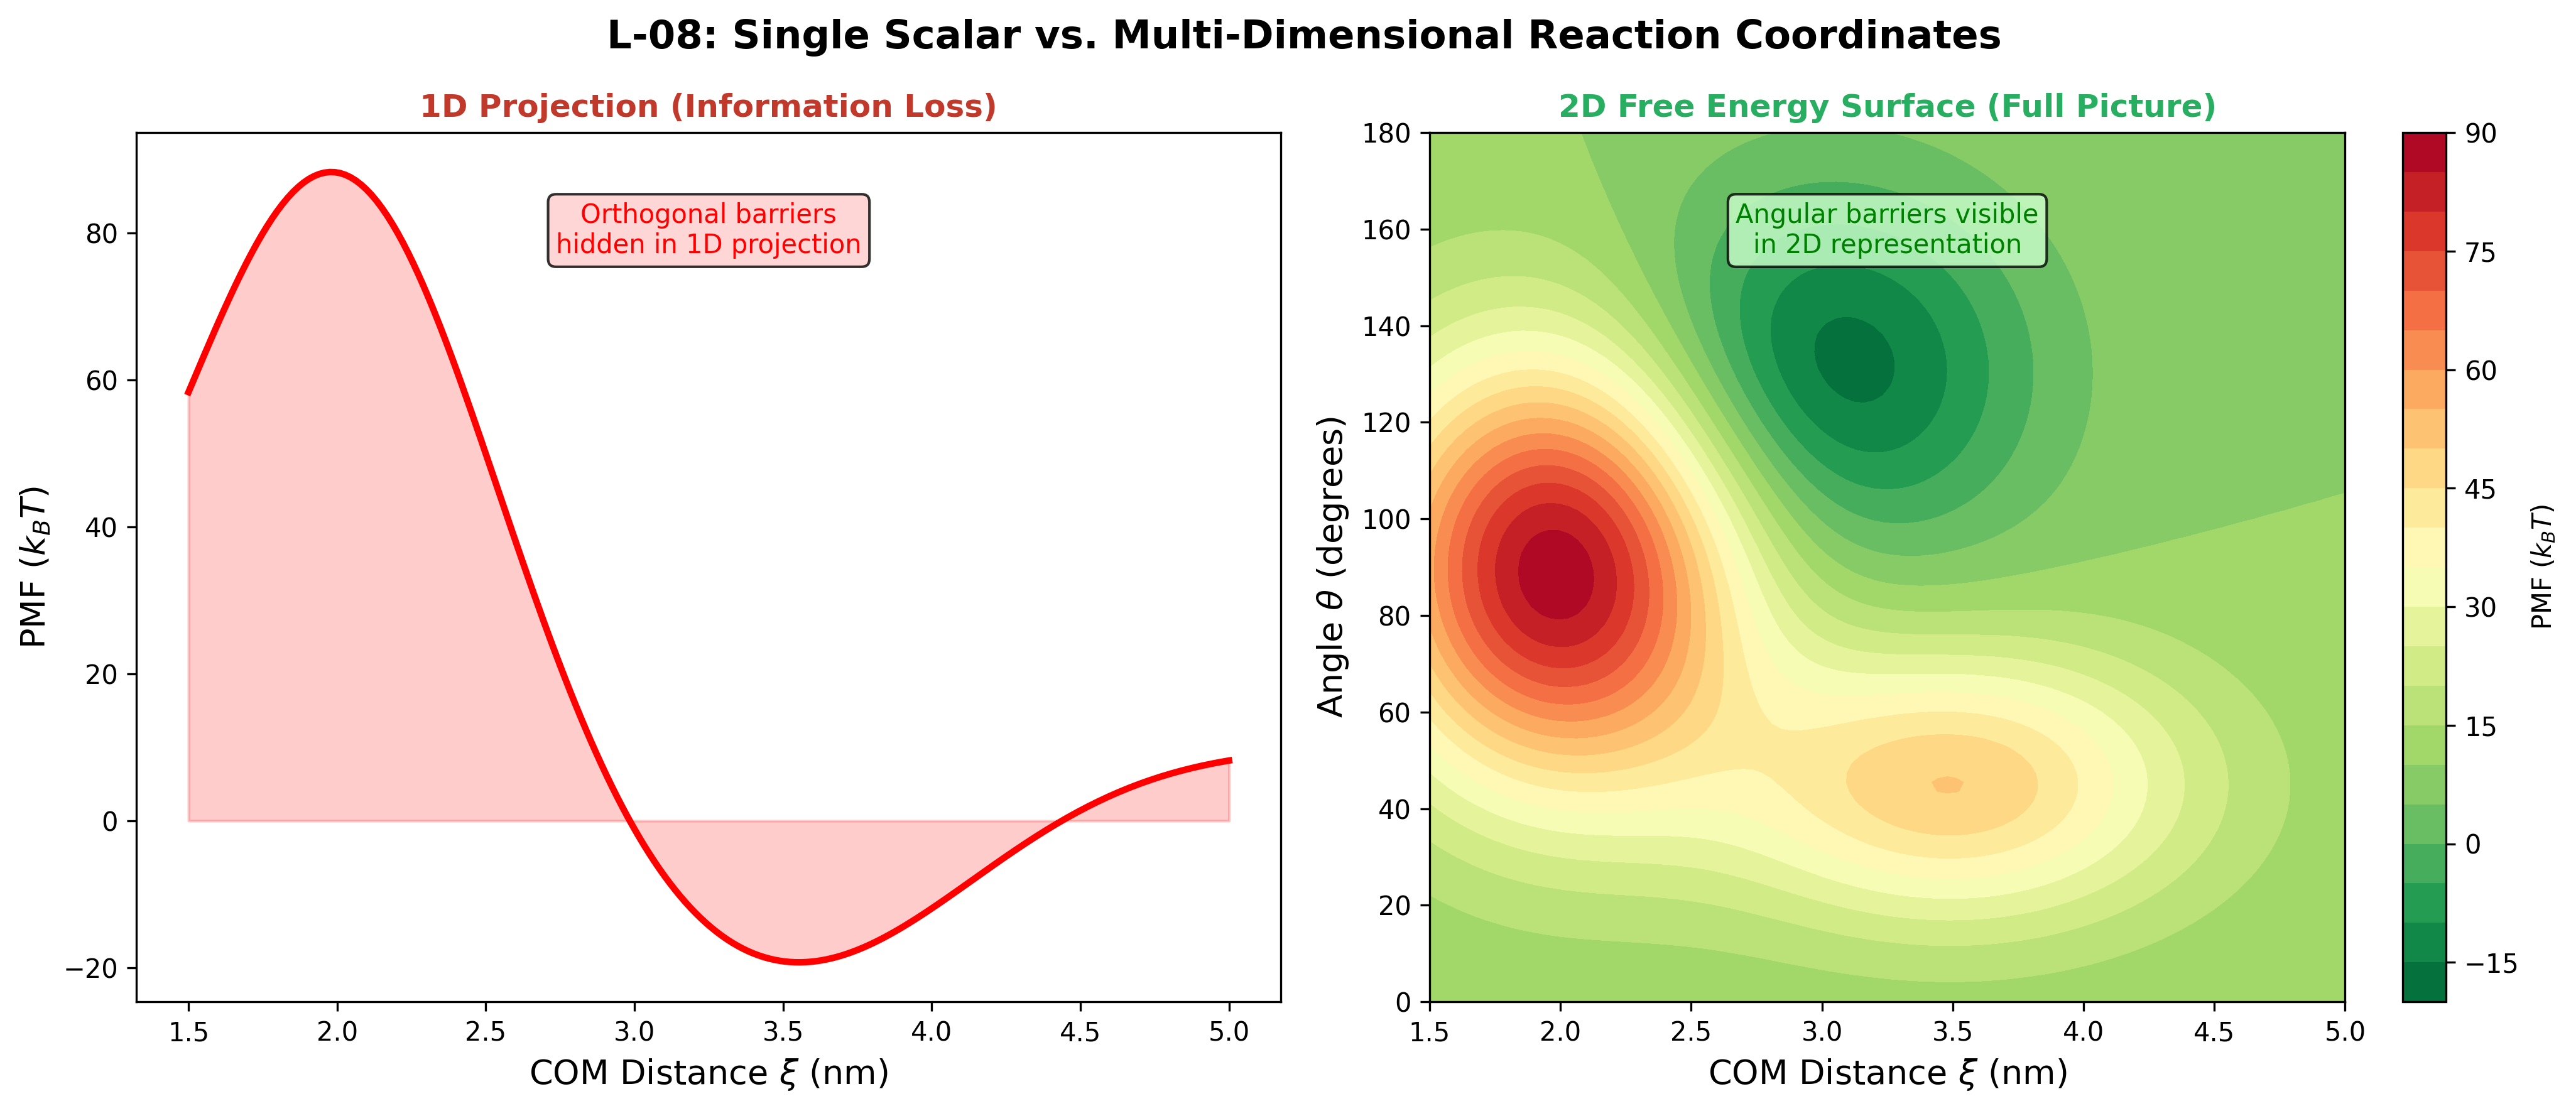
\includegraphics[width=\columnwidth]{L-08_reaction_coordinate_dimensionality}
  \caption{Multi-dimensional collective variable framework.  Protein
  unbinding is characterized by three complementary CVs: COM distance
  $\xi$, angular deviation $\theta$, and interface contact fraction $Q$.
  The combined CV space resolves rotational and conformational unbinding
  pathways that a scalar COM distance alone cannot capture.}
  \label{fig:multidim_cv}
\end{figure}

\subsection{Well-Tempered Metadynamics}\label{sec:metadynamics}

Well-tempered metadynamics~\cite{barducci2008} provides an independent
cross-validation of the PMF by depositing history-dependent Gaussian
bias potentials along the collective variable:
\begin{equation}\label{eq:metad_bias}
  V_{\mathrm{bias}}(\xi, t) = \sum_{t'<t} w(t')
  \exp\!\left(-\frac{(\xi - \xi(t'))^2}{2\sigma^2}\right)
\end{equation}
where the Gaussian height decays as the bias accumulates:
\begin{equation}\label{eq:metad_tempering}
  w(t) = w_0 \exp\!\left(
    -\frac{V_{\mathrm{bias}}(\xi(t), t)}{k_B \Delta T}
  \right).
\end{equation}
The bias factor $\gamma = (T + \Delta T) / T$ controls the trade-off
between exploration speed and accuracy.  The converged free energy surface
is recovered as
\begin{equation}\label{eq:metad_fes}
  G(\xi) = -\frac{\gamma}{\gamma - 1}\,V_{\mathrm{bias}}(\xi, t \to \infty) + C.
\end{equation}
Convergence is monitored by computing
$\max_\xi |G(\xi, t) - G(\xi, t - \Delta t_{\mathrm{check}})| < \epsilon$,
with $\epsilon = 1.0$~kJ/mol as the default tolerance.  The implementation
uses OpenMM's native \texttt{Metadynamics} class with parameters:
$w_0 = 1.0$~kJ/mol, $\sigma = 0.05$~nm, deposition interval 1.0~ps,
$\gamma = 15$, and 50~ns simulation duration (Fig.~\ref{fig:metadynamics}).

\begin{figure}[H]
  \centering
  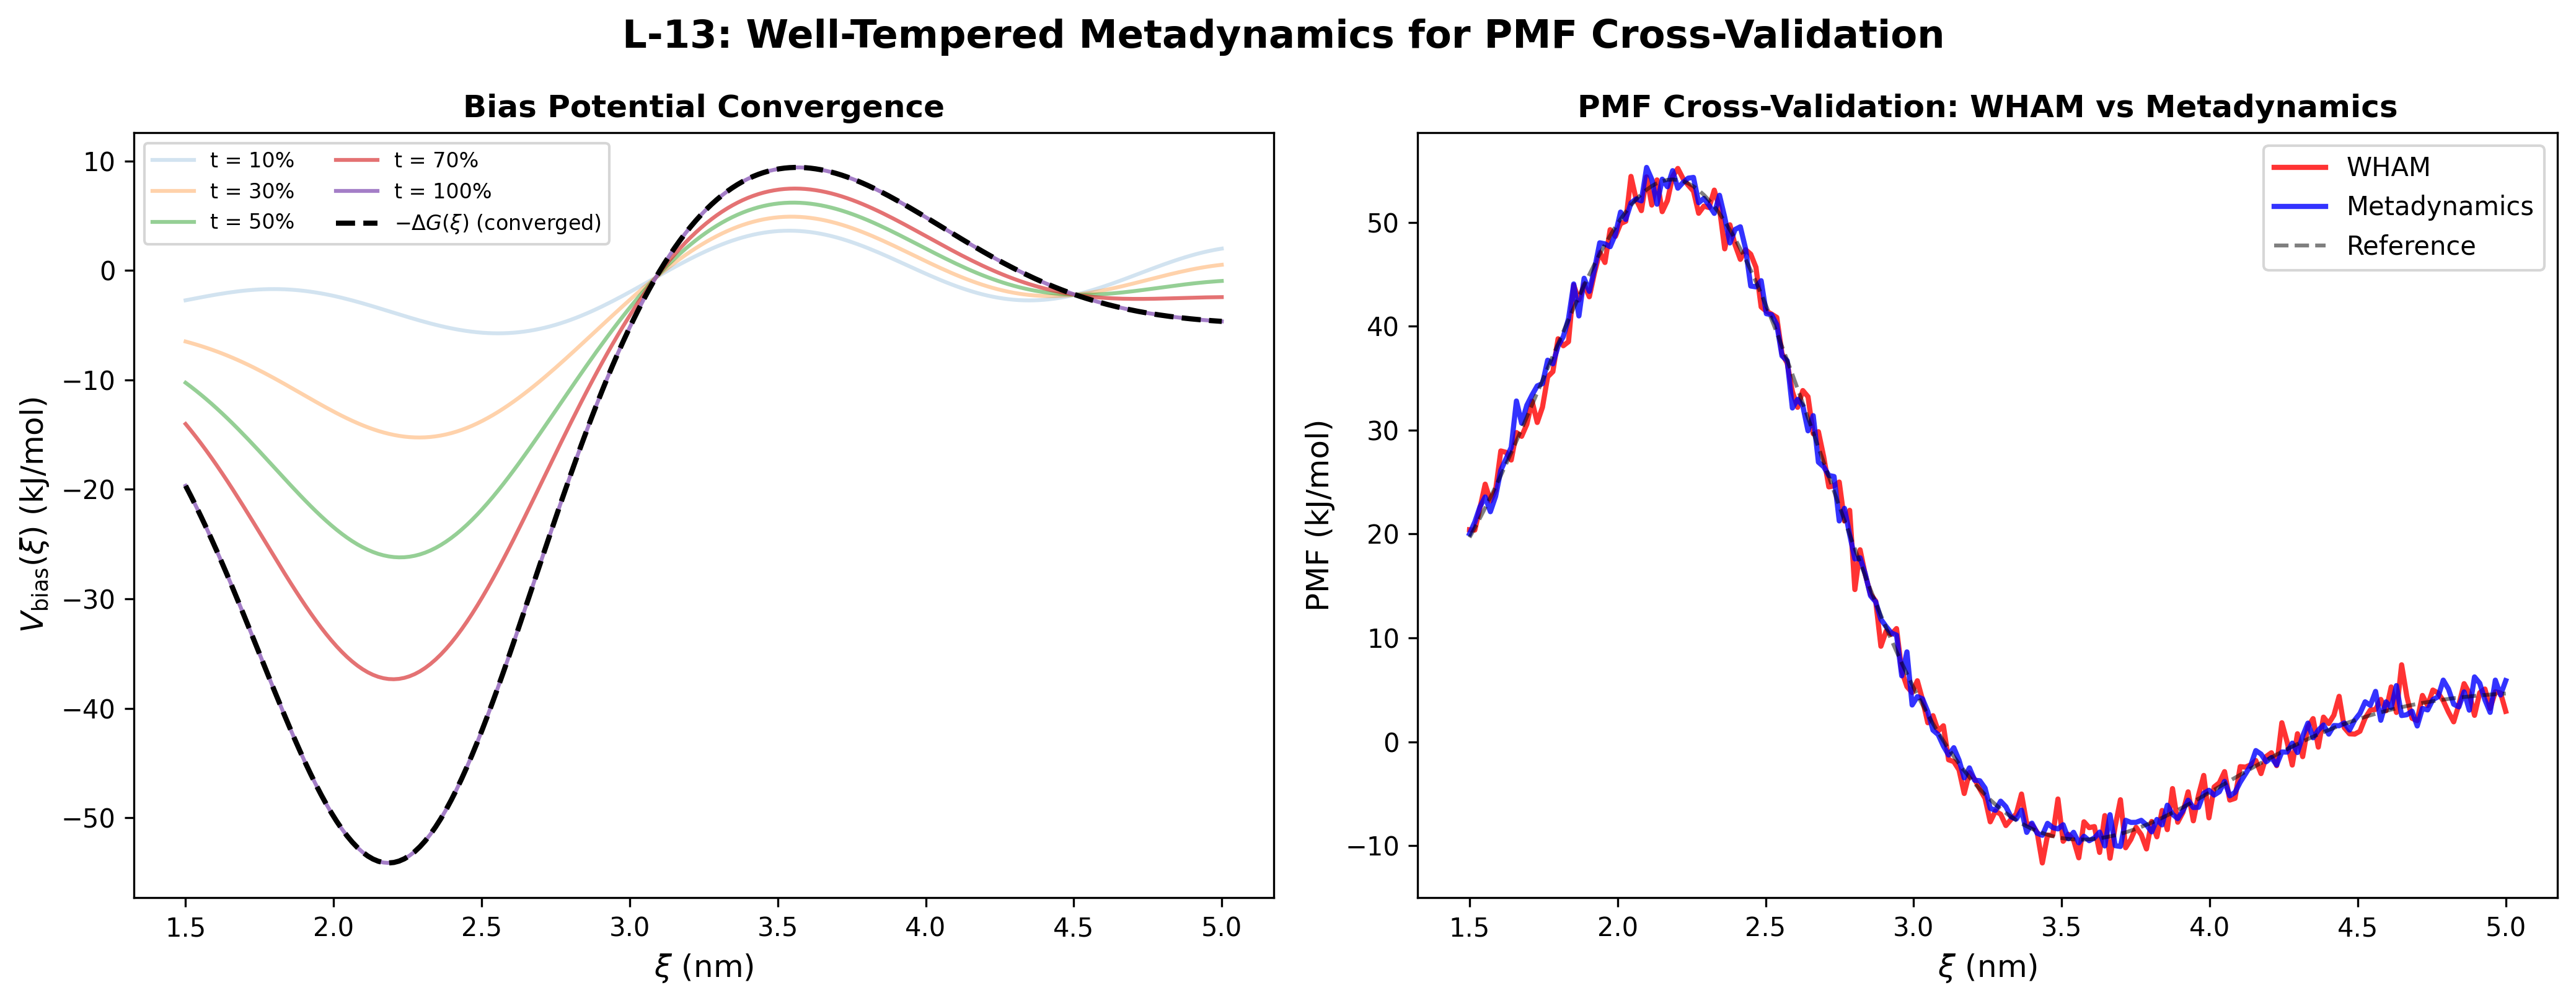
\includegraphics[width=\columnwidth]{L-13_metadynamics_convergence}
  \caption{Well-tempered metadynamics convergence.  Gaussian bias deposits
  fill free energy minima over time, with height decay controlled by the
  bias factor $\gamma$.  The free energy surface converges as the bias
  potential reaches a steady state, providing cross-validation of
  WHAM-derived PMF profiles.}
  \label{fig:metadynamics}
\end{figure}

\subsection{Alchemical Free Energy Perturbation}\label{sec:fep}

To enable computational mutagenesis studies, the pipeline implements
alchemical free energy perturbation (FEP) based on a thermodynamic cycle
that decomposes the mutation-induced binding free energy change as
\begin{equation}\label{eq:ddg}
  \Delta\Delta G = \Delta G_{\mathrm{alch,complex}}
    - \Delta G_{\mathrm{alch,free}}
\end{equation}
where $\Delta G_{\mathrm{alch,complex}}$ and $\Delta G_{\mathrm{alch,free}}$
are computed by alchemically transforming the wild-type residue to the
mutant in the bound complex and free protein, respectively.

The alchemical transformation is parameterized by a coupling parameter
$\lambda \in [0, 1]$ with the hybrid Hamiltonian
\begin{equation}\label{eq:alch_hamiltonian}
  H(\lambda) = (1-\lambda)\,H_{\mathrm{WT}} + \lambda\,H_{\mathrm{Mut}}
    + H_{\mathrm{env}}.
\end{equation}
To avoid singularities in the Lennard-Jones potential at
$\lambda = 0$ or $\lambda = 1$ when atoms are created or annihilated,
soft-core potentials are employed~\cite{gapsys2015}:
\begin{equation}\label{eq:softcore}
  U_{\mathrm{LJ}}^{\mathrm{soft}}(r; \lambda) = 4\epsilon\!\left[
    \left(\frac{\sigma^2}
      {\alpha_{\mathrm{LJ}} \sigma^2 \lambda^p + r^2}\right)^{\!6}
    - \left(\frac{\sigma^2}
      {\alpha_{\mathrm{LJ}} \sigma^2 \lambda^p + r^2}\right)^{\!3}
  \right]
\end{equation}
with $\alpha_{\mathrm{LJ}} = 0.5$ and soft-core power $p = 1$.  Free
energy differences between adjacent $\lambda$ windows are computed using
BAR, and global analysis across all 20 $\lambda$ windows employs
MBAR~\cite{shirts2008} (Fig.~\ref{fig:fep_cycle}).

\begin{figure}[H]
  \centering
  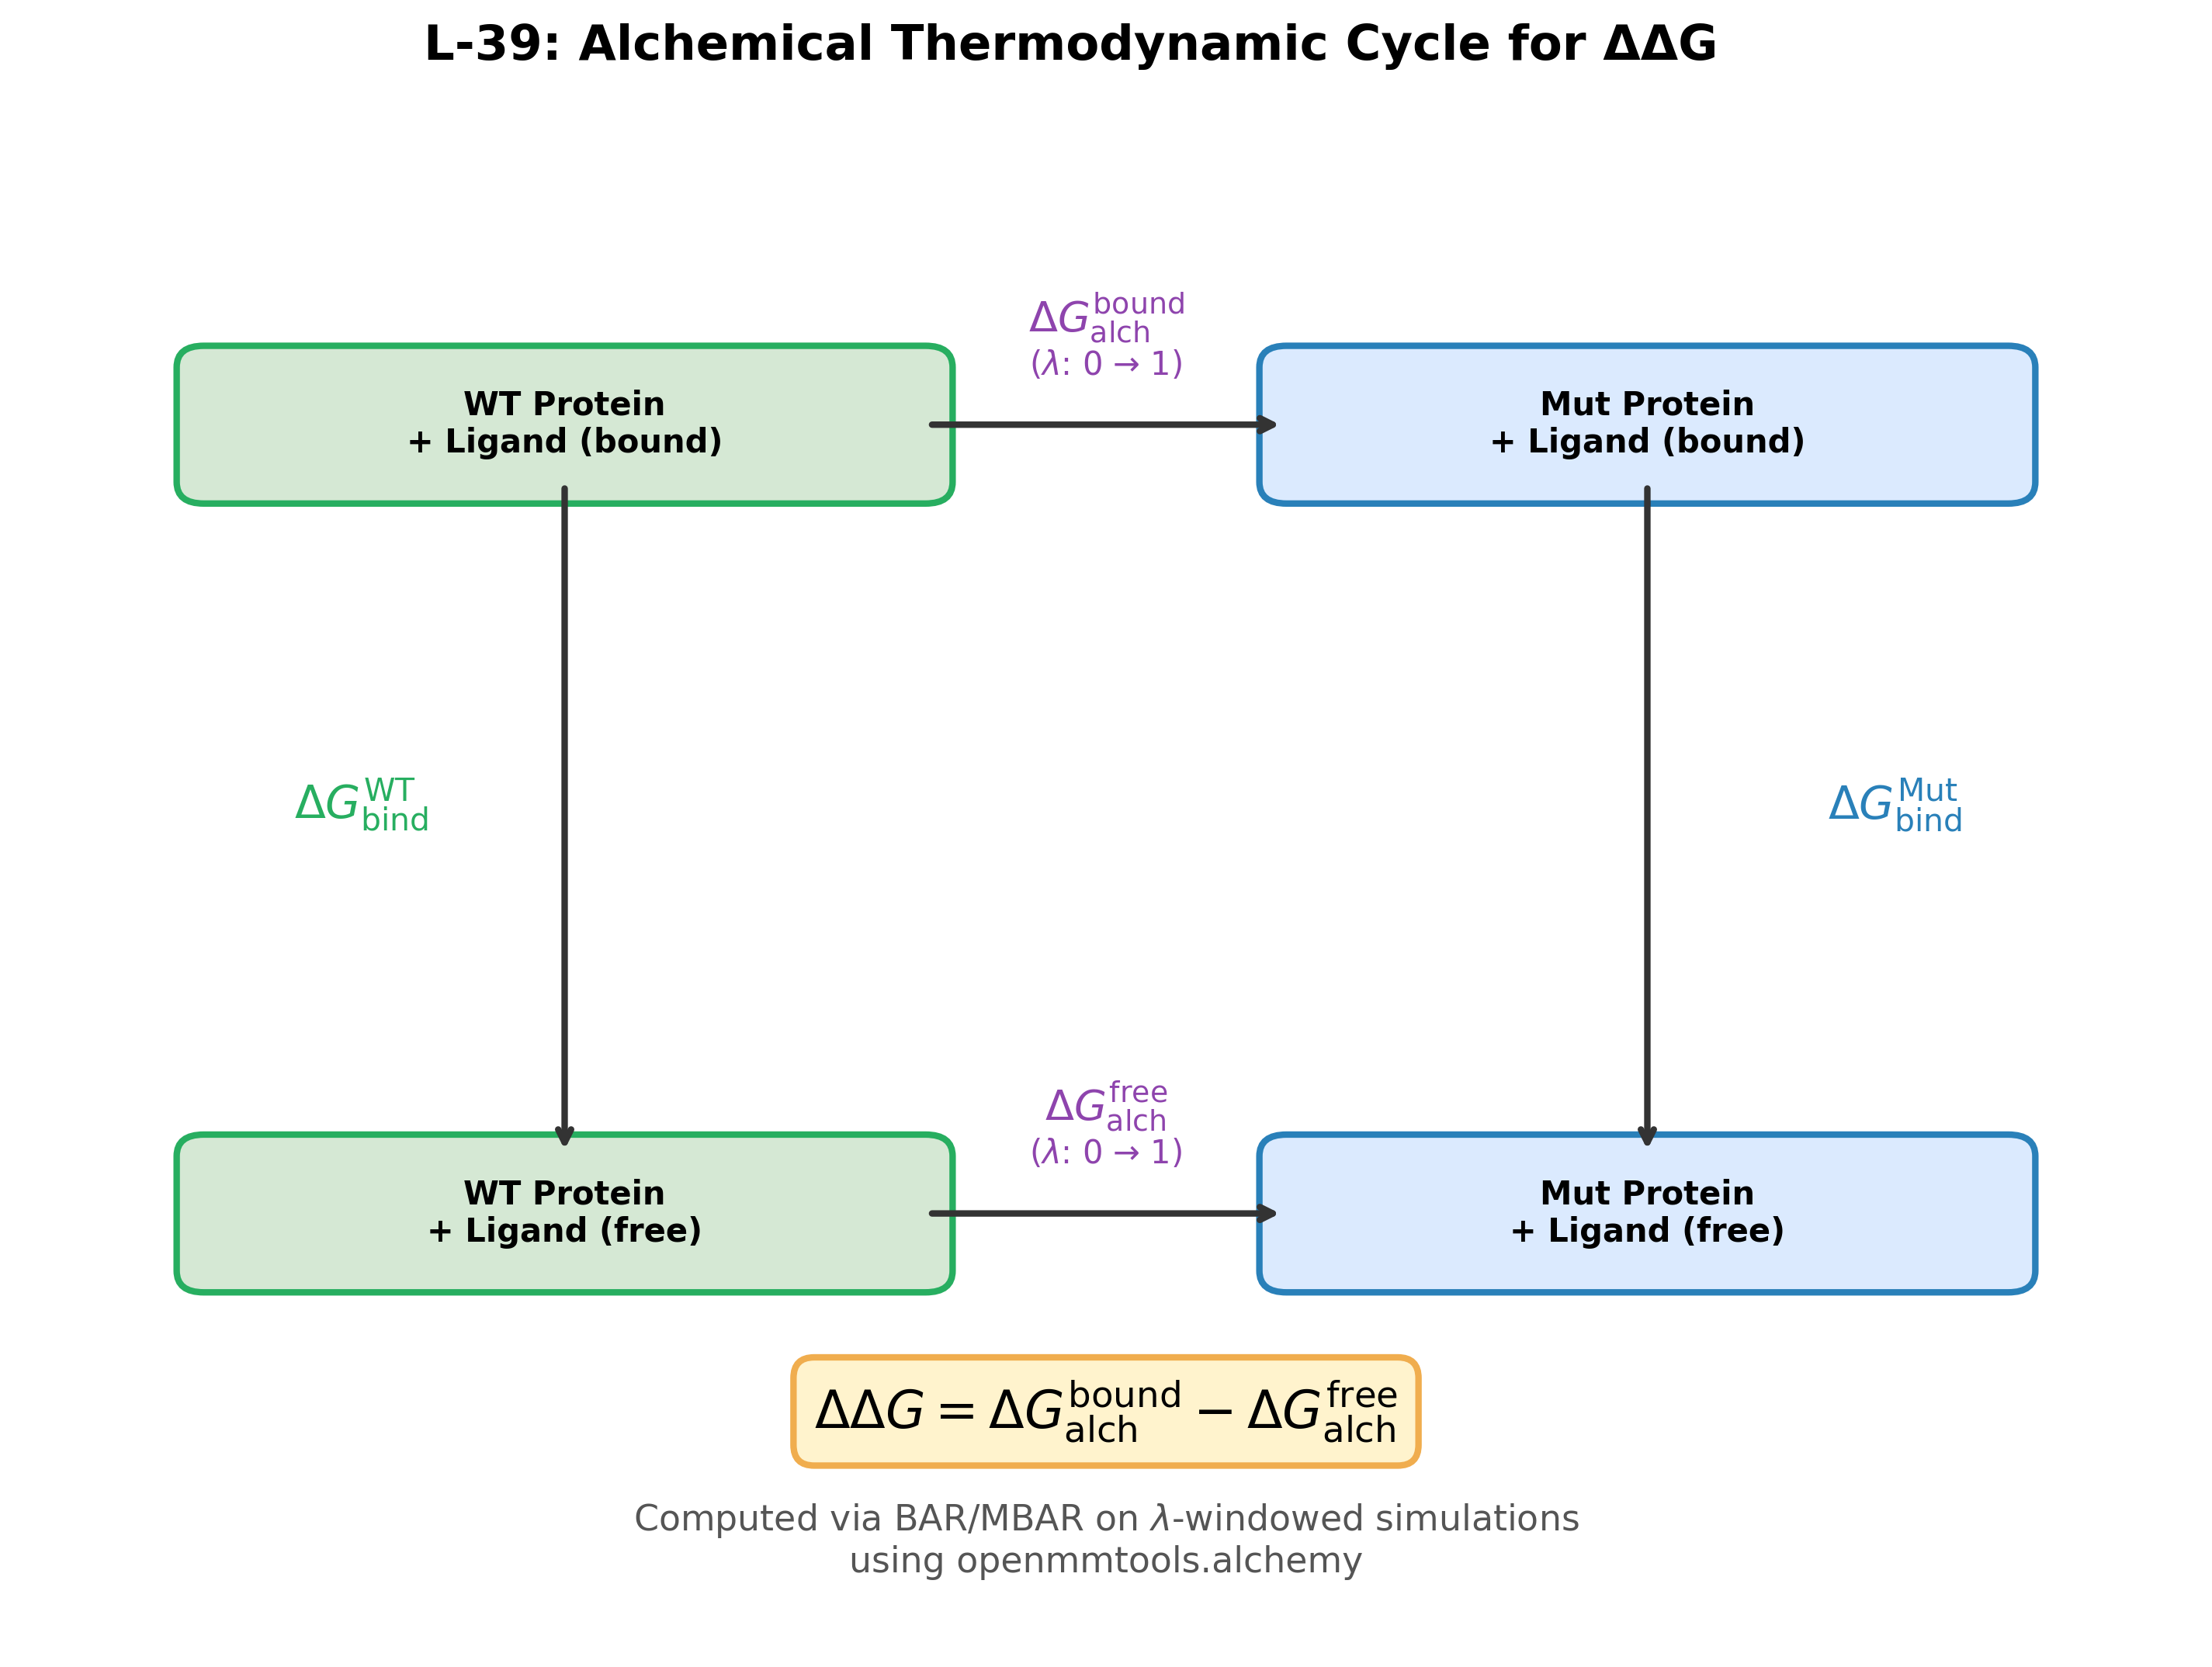
\includegraphics[width=\columnwidth]{L-39_alchemical_thermodynamic_cycle}
  \caption{Alchemical thermodynamic cycle for computing mutational
  $\Delta\Delta G$.  The vertical legs represent physical binding
  processes; the horizontal legs represent alchemical wild-type to mutant
  transformations parameterized by $\lambda$.  The cycle closure condition
  $\Delta\Delta G = \Delta G_{\mathrm{alch,complex}} -
  \Delta G_{\mathrm{alch,free}}$ follows from thermodynamic path
  independence.}
  \label{fig:fep_cycle}
\end{figure}

\subsection{Markov State Model Construction}\label{sec:msm}

The pipeline constructs Markov State Models (MSMs) from production
trajectories to extract kinetic information---association and dissociation
rates ($k_{\mathrm{on}}$, $k_{\mathrm{off}}$) and mean first passage times
(MFPTs)---that complement the thermodynamic $\Delta G$ from enhanced
sampling~\cite{noe2009,prinz2011}.  Trajectories are featurized using
backbone dihedral angles represented as $[\sin\phi, \cos\phi, \sin\psi,
\cos\psi]$ pairs combined with interface contact distances.
Dimensionality reduction via Time-lagged Independent Component Analysis
(TICA)~\cite{perez2013} identifies the slowest order parameters:
\begin{equation}\label{eq:tica}
  \mathbf{C}(\tau)\,\mathbf{v}_k = \lambda_k\,\mathbf{C}(0)\,\mathbf{v}_k.
\end{equation}
The projected data are clustered into $N_c = 200$ microstates, and the
row-stochastic transition matrix at lag time $\tau$ is estimated as
$T_{ij}(\tau) = C_{ij}(\tau) / \sum_k C_{ik}(\tau)$.  Implied timescales
$t_k = -\tau / \ln \mu_k$ are computed from the eigenvalues $\mu_k$ of
$\mathbf{T}$ and validated for convergence across a range of lag times
(1--500~ps).  A Bayesian MSM with 100 posterior samples provides
uncertainty estimates on all kinetic quantities (Fig.~\ref{fig:msm}).

\begin{figure}[H]
  \centering
  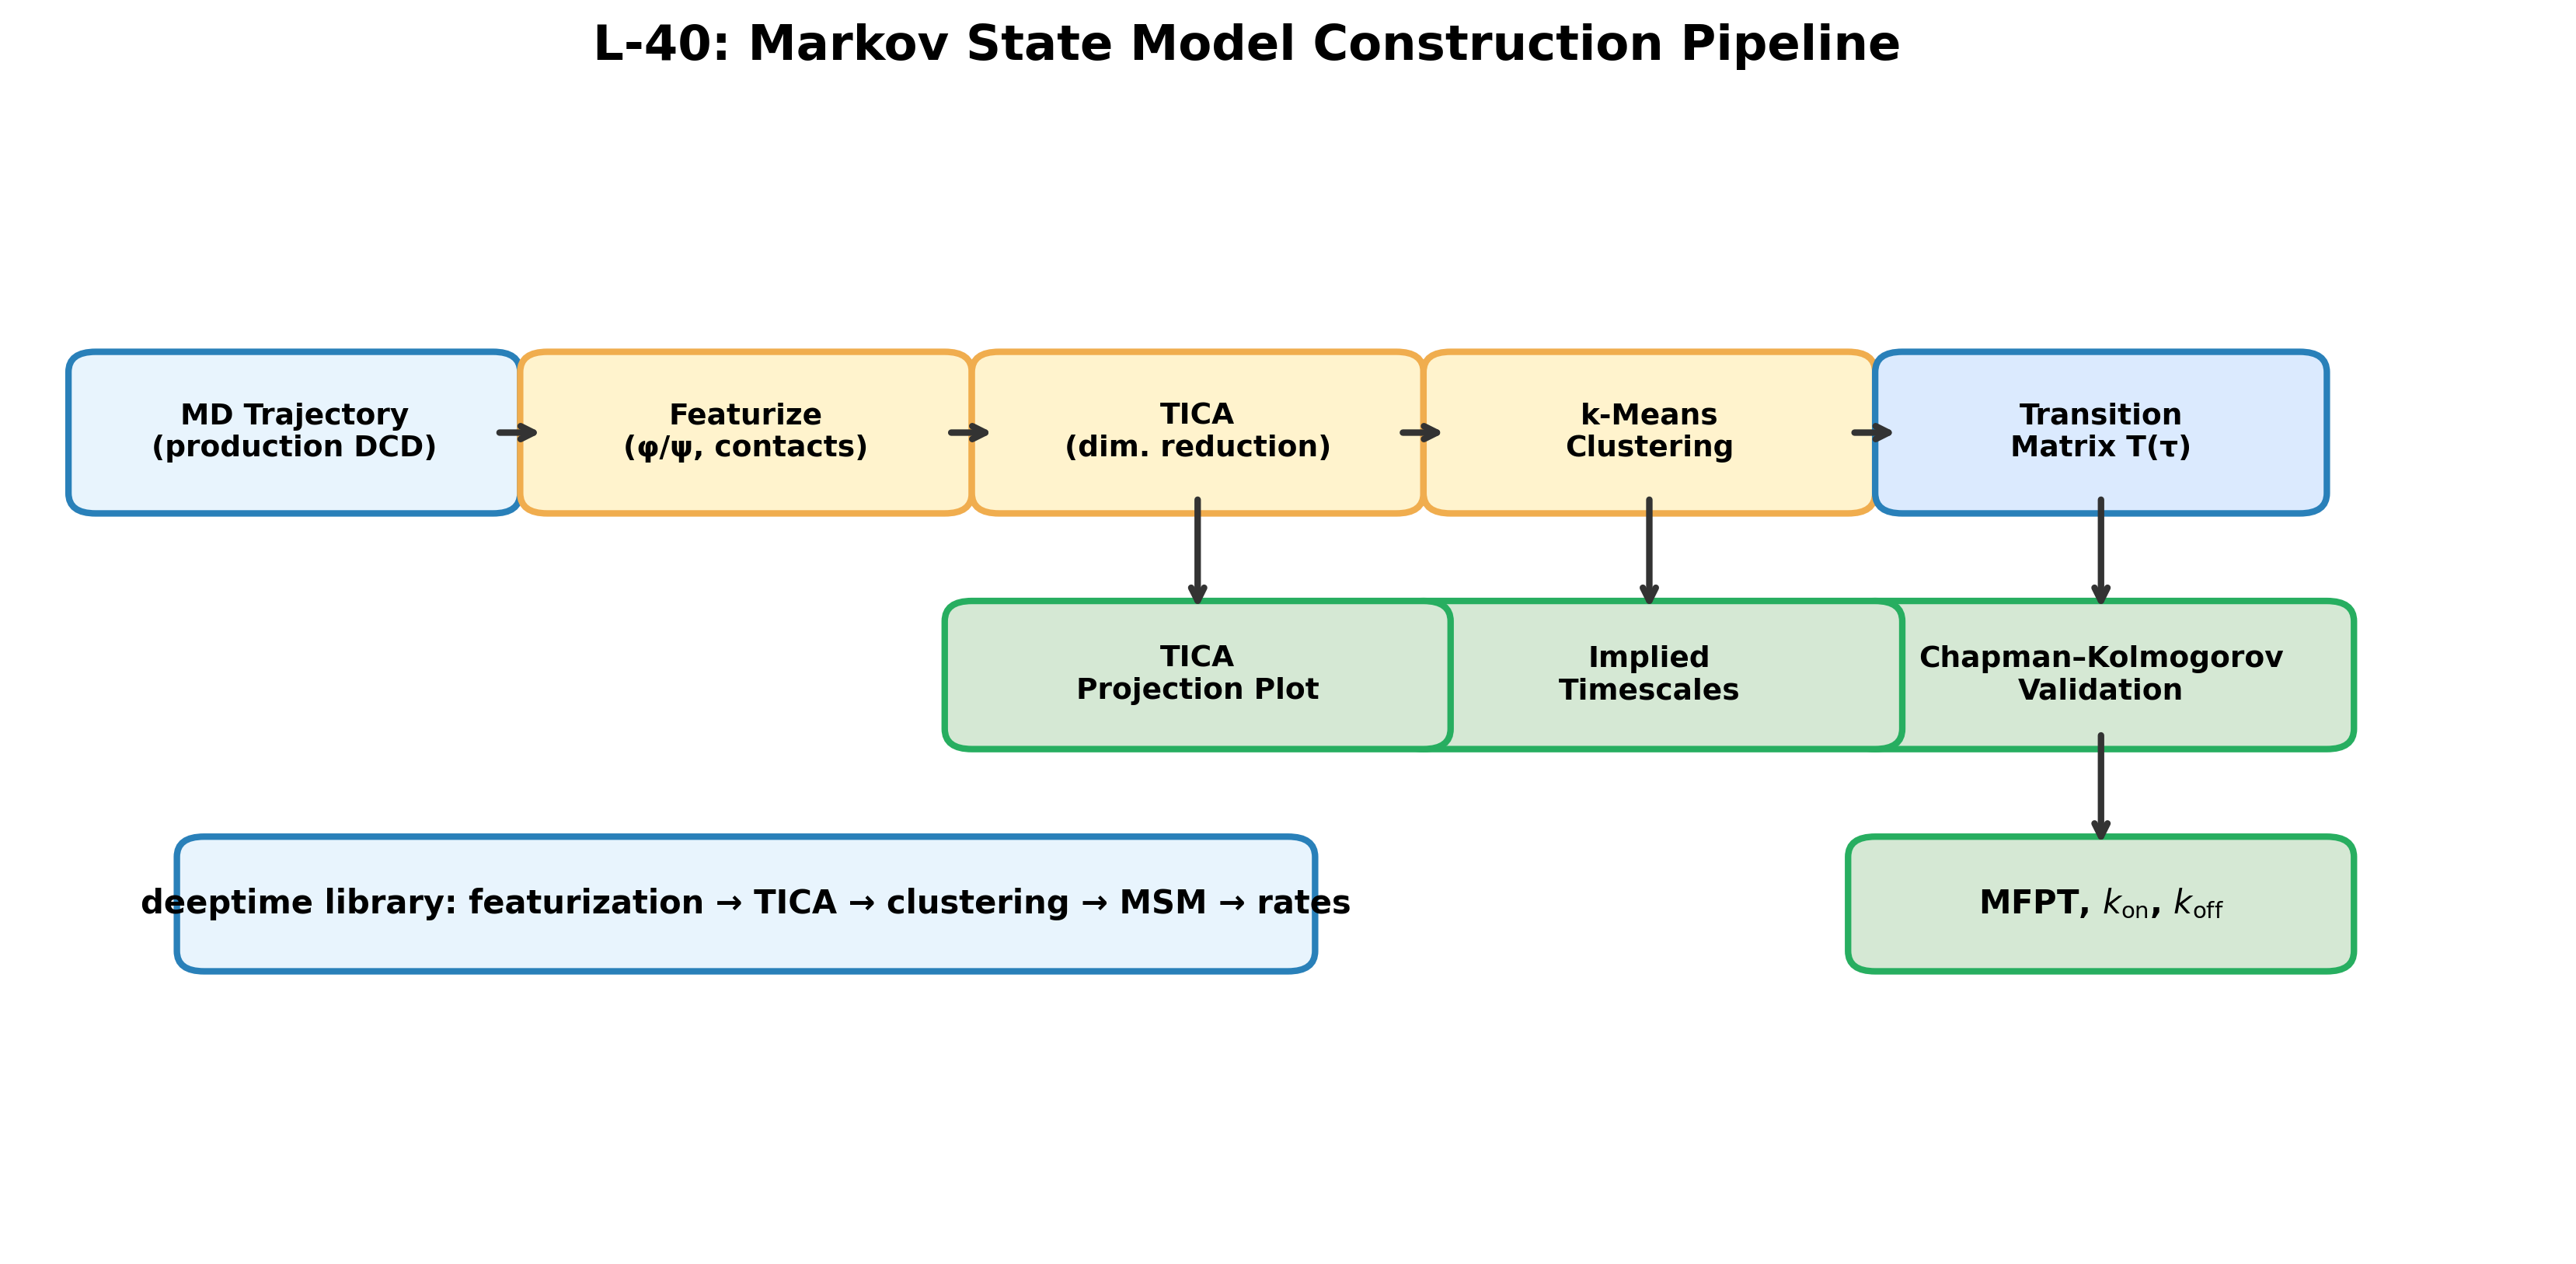
\includegraphics[width=\columnwidth]{L-40_msm_construction_pipeline}
  \caption{MSM construction pipeline.  Production trajectories are
  featurized (backbone dihedrals + contact distances), projected via TICA
  into the slowest order parameters, clustered into microstates, and
  used to estimate a transition matrix $\mathbf{T}(\tau)$.  Implied
  timescale convergence validates the Markov assumption, and coarse-grained
  kinetic models yield $k_{\mathrm{on}}$, $k_{\mathrm{off}}$, and MFPTs.}
  \label{fig:msm}
\end{figure}

\subsection{Finite-Size Electrostatic Corrections}\label{sec:finite_size}

Periodic boundary conditions with PME introduce systematic electrostatic
artifacts from self-interaction with periodic images, with errors on the
order of 1--2~kcal/mol for charged protein-protein
systems~\cite{huenberger1999,rocklin2013}---comparable to the target
$\Delta G_{\mathrm{bind}}$ accuracy.  The H\"unenberger-McCammon
correction for a net charge $Q$ in a cubic box of edge length $L$ is
\begin{equation}\label{eq:hm_correction}
  \Delta G_{\mathrm{HM}} = -\frac{Q^2 \cdot \xi_{\mathrm{EW}} \cdot k_e}
    {2\,\epsilon_s\,L}
\end{equation}
where $\xi_{\mathrm{EW}} \approx -2.837297$ is the Madelung constant for
a simple cubic lattice, $k_e = 138.935456$~kJ$\cdot$nm/(mol$\cdot$e$^2$),
and $\epsilon_s \approx 80$ is the solvent dielectric at 310~K.  The
Rocklin correction~\cite{rocklin2013} extends this to include quadrupole
contributions.  Additionally, the pipeline supports extrapolation to the
infinite-box limit by fitting the electrostatic energy as a function of
box size to $E(L) = E_\infty + a/L + b/L^3$
(Fig.~\ref{fig:finite_size}).

\begin{figure}[H]
  \centering
  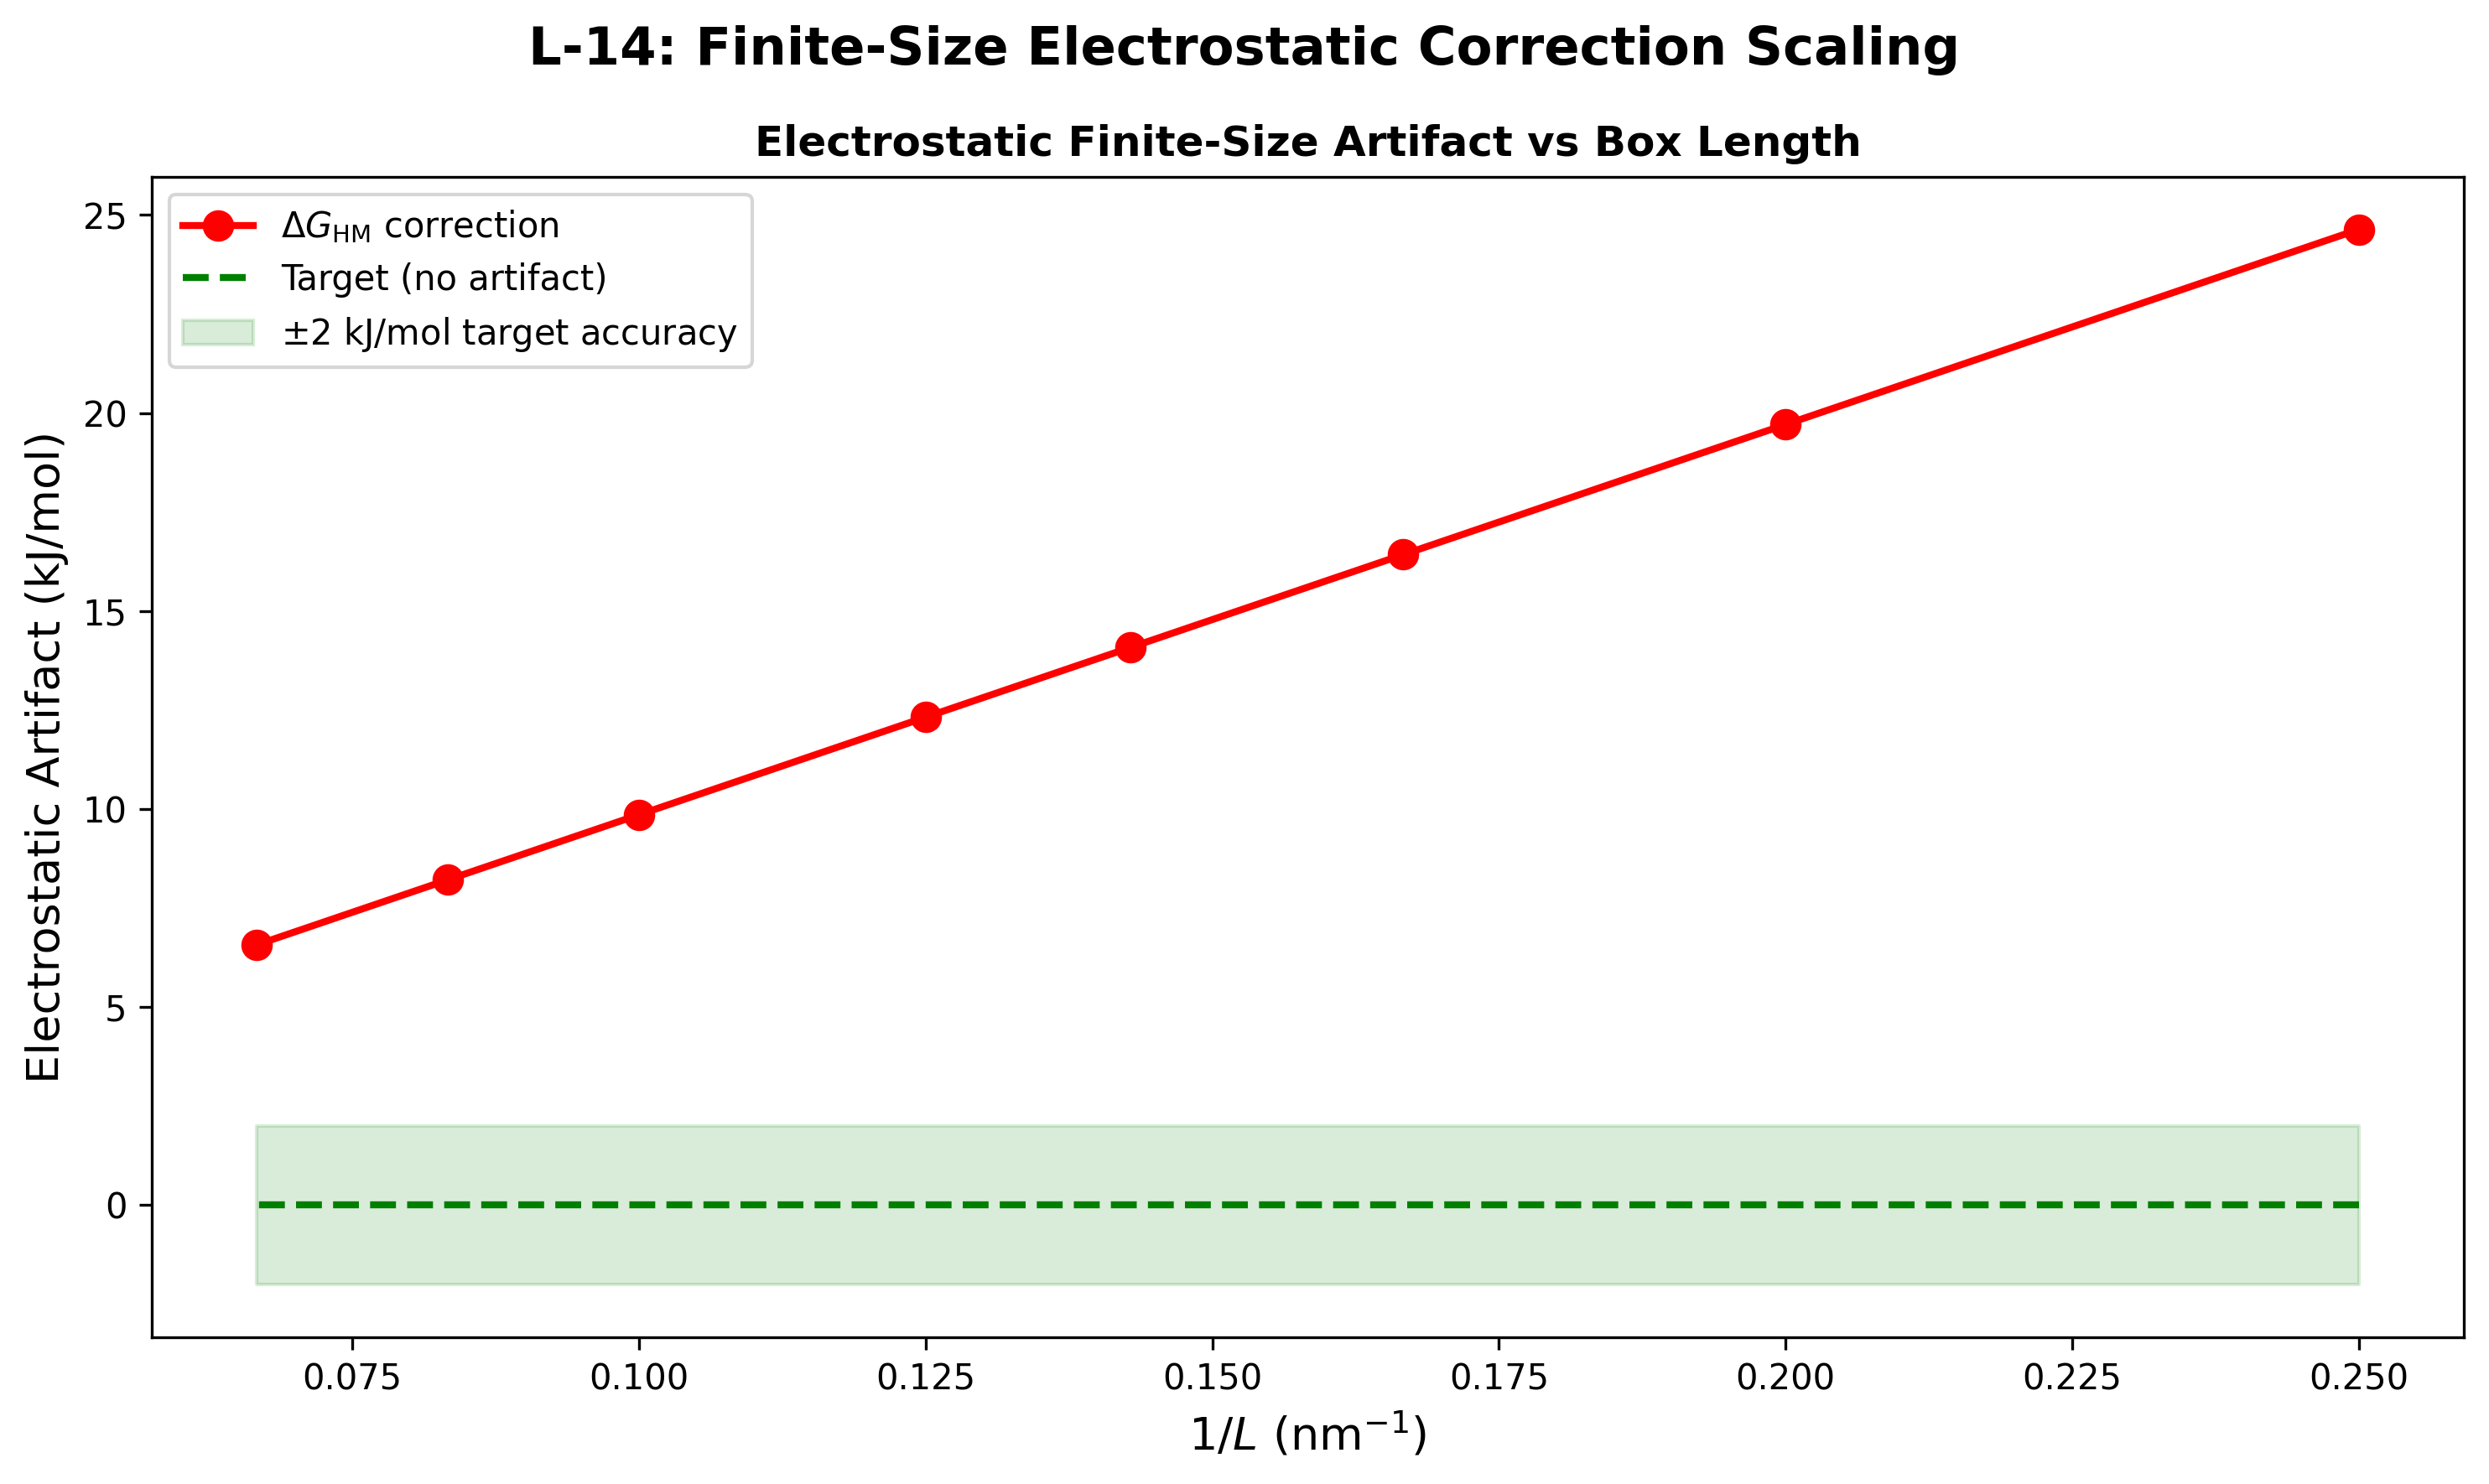
\includegraphics[width=\columnwidth]{L-14_finite_size_correction}
  \caption{Finite-size electrostatic correction.  The H\"unenberger-McCammon
  and Rocklin corrections remove systematic artifacts from periodic image
  interactions in PME simulations.  The magnitude of the correction scales
  as $1/L$ and becomes significant ($>1$~kcal/mol) for box sizes typical
  of protein-protein complex simulations.}
  \label{fig:finite_size}
\end{figure}

% ============================================================
\section{Software Architecture}\label{sec:architecture}

\subsection{Modular Design}\label{sec:modules}

The pipeline is organized into five primary subsystems---preparation,
simulation, analysis, physics, and visualization---each encapsulated in its
own Python subpackage under \texttt{src/} (Table~\ref{tab:modules}).

\begin{table}[H]
  \centering
  \caption{Pipeline Module Organization}
  \label{tab:modules}
  \begin{tabular}{@{}lp{5.2cm}@{}}
    \toprule
    \textbf{Subpackage} & \textbf{Modules} \\
    \midrule
    \texttt{prep/} & \texttt{pdb\_fetch}, \texttt{pdb\_clean},
      \texttt{protonate}, \texttt{topology}, \texttt{solvate} \\
    \texttt{simulate/} & \texttt{minimizer}, \texttt{equilibrate},
      \texttt{production}, \texttt{smd}, \texttt{umbrella} \\
    \texttt{analyze/} & \texttt{trajectory}, \texttt{structural},
      \texttt{contacts}, \texttt{wham}, \texttt{jarzynski},
      \texttt{convergence} \\
    \texttt{physics/} & \texttt{collective\_variables},
      \texttt{restraints}, \texttt{units} \\
    \texttt{visualization/} & \texttt{viewer\_3d}, \texttt{plot\_pmf},
      \texttt{plot\_timeseries} \\
    \bottomrule
  \end{tabular}
\end{table}

All simulation parameters are centralized in a single configuration module
(\texttt{src/config.py}) that serves as the sole source of truth for
physical constants and algorithmic parameters.  No magic numbers appear
elsewhere in the codebase.  Key configuration objects---\texttt{SystemConfig},
\texttt{MinimizationConfig}, \texttt{EquilibrationConfig},
\texttt{ProductionConfig}, \texttt{SMDConfig}, \texttt{UmbrellaConfig}, and
\texttt{WHAMConfig}---are implemented as frozen (immutable) Python
dataclasses decorated with \texttt{@dataclass(frozen=True)}, which prevents
accidental parameter modification during execution.

\subsection{Internal Unit System}\label{sec:units}

All internal computations follow the OpenMM unit convention: lengths in
nanometers, time in picoseconds, mass in atomic mass units, energy in
kJ/mol, temperature in Kelvin, charge in elementary units, and force in
kJ/mol/nm.  Conversions to commonly used units (e.g., \AA, kcal/mol, ns)
are provided via \texttt{src/physics/units.py}, with the critical
conversion factor $1~\mathrm{kcal/mol} = 4.184~\mathrm{kJ/mol}$ used for
final $\Delta G$ reporting.

\subsection{Exception Hierarchy}\label{sec:exceptions}

The pipeline implements a domain-specific exception hierarchy rooted in
\texttt{PipelineError}, replacing all \texttt{assert}-based validation
(which is silently removed under \texttt{python~-O}) with proper
exception raising that is never optimized away:
\begin{itemize}
  \item \texttt{PhysicalValidityError}: raised when a physical invariant
    (IV-1 through IV-10) is violated, halting the pipeline.
  \item \texttt{ConvergenceError}: raised when an iterative solver (e.g.,
    WHAM) fails to converge within the allowed iteration limit.
  \item \texttt{InsufficientSamplingError}: raised when sampling quality
    criteria (e.g., histogram overlap) are not met.
\end{itemize}
All nine original \texttt{assert} statements across the analysis modules
(\texttt{contacts.py}, \texttt{convergence.py}, \texttt{wham.py}) have been
replaced with explicit \texttt{if not condition: raise ValueError(msg)}
guards that provide descriptive error messages including actual vs.\
expected array shapes.

\subsection{Configuration and Fault Tolerance}\label{sec:config_v2}

The centralized configuration system has been extended with YAML/JSON
file support, enabling parameter specification via configuration files
rather than source code modification.  A three-tier precedence hierarchy
(command-line arguments $>$ configuration file $>$ frozen dataclass
defaults) ensures flexibility while maintaining the safety guarantees
of immutable defaults.

Long-running simulations are protected by a checkpoint-based
fault-tolerance system: simulation state is periodically serialized to
disk, and the pipeline detects existing checkpoints on restart, resuming
from the last valid snapshot rather than repeating computation from the
beginning.

\subsection{Platform Selection}\label{sec:platform}

The pipeline automatically selects the optimal OpenMM compute platform at
runtime using a prioritized detection scheme (CUDA $>$ OpenCL $>$ CPU),
replacing the previous CPU-only hardcoding.  GPU acceleration reduces
wall-clock time by approximately two orders of magnitude for production-
scale systems ($N > 50{,}000$ atoms), making the 100~ns equilibrium and
50-replicate SMD campaigns feasible within practical timeframes
(Fig.~\ref{fig:platform}).

\begin{figure}[H]
  \centering
  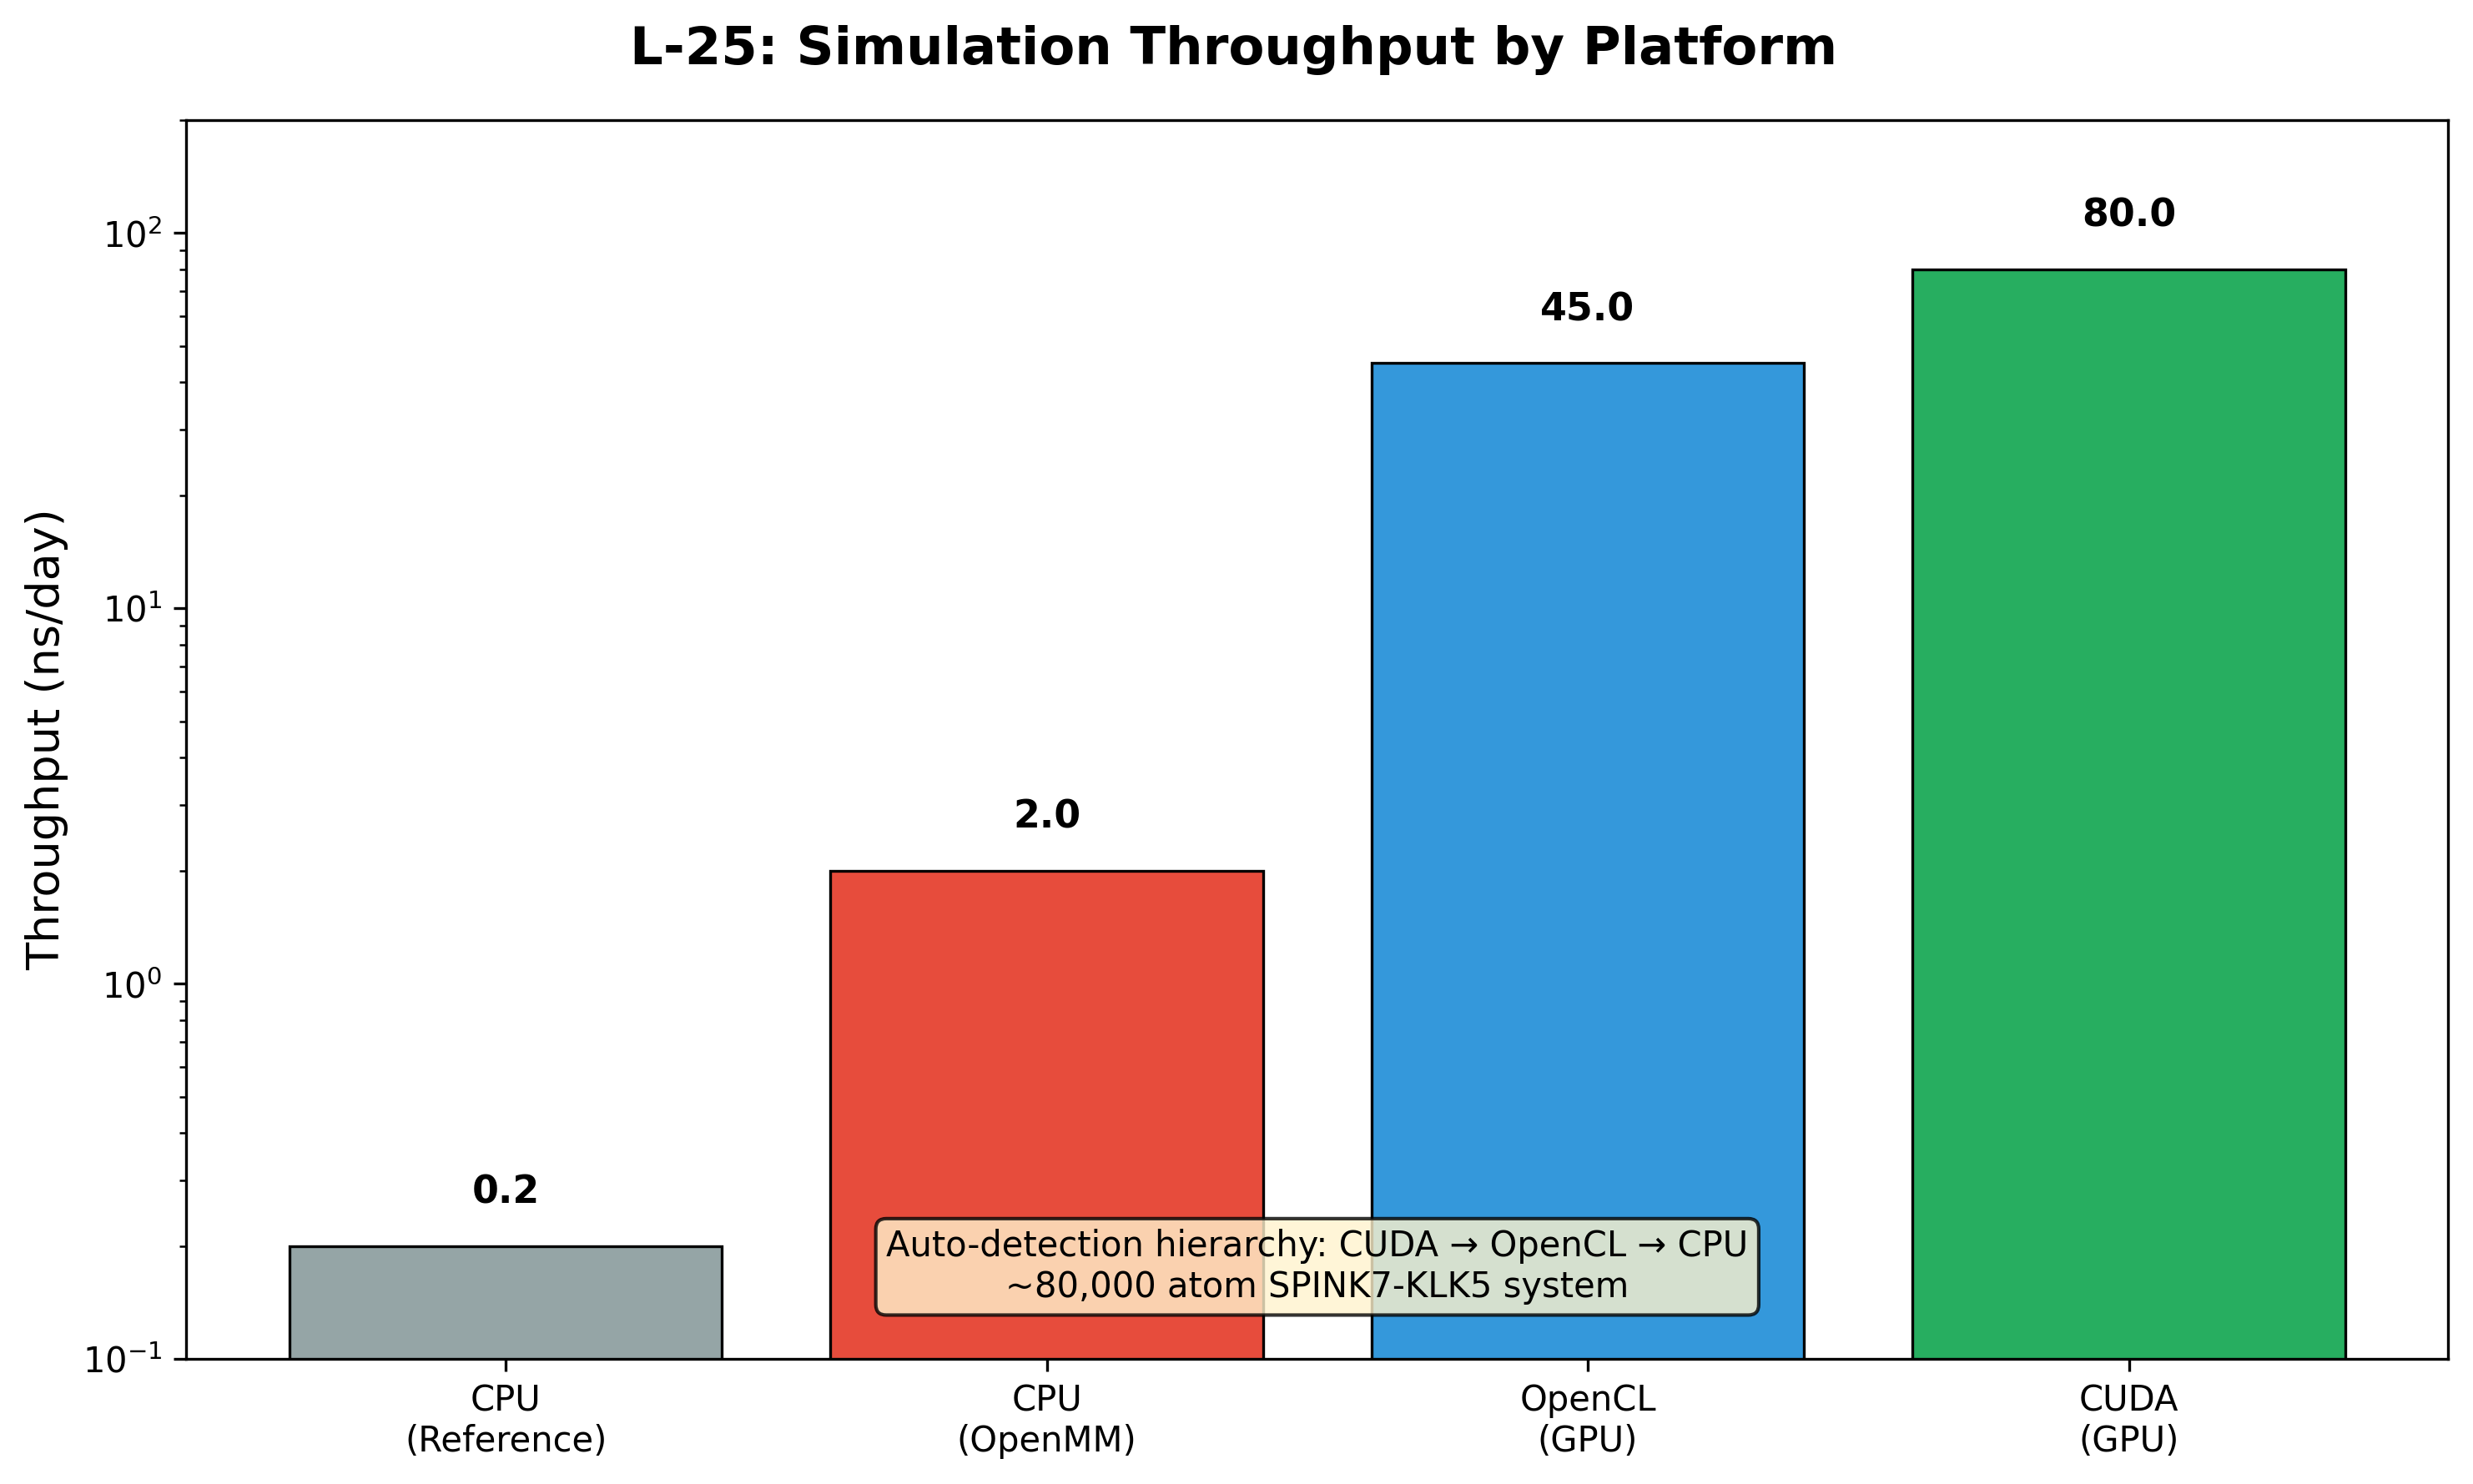
\includegraphics[width=\columnwidth]{L-25_platform_throughput}
  \caption{Compute platform throughput comparison.  GPU acceleration via
  CUDA provides approximately 100$\times$ speedup over CPU for
  production-scale systems, enabling practical execution of
  multi-nanosecond campaigns.}
  \label{fig:platform}
\end{figure}

\subsection{Memory Management}\label{sec:memory}

MD trajectories can reach tens of gigabytes on disk.  The pipeline enforces
strict memory management: frames are written incrementally to disk via
OpenMM's \texttt{DCDReporter} during simulation and loaded in chunks via
\texttt{mdtraj.iterload()} during analysis; NumPy arrays for timeseries
data are preallocated to their known final size (repeated
\texttt{np.append()} calls are prohibited); and trajectories exceeding 1~GB
are analyzed in configurable chunks (default: 100~frames) with running
statistics to prevent out-of-memory errors.  Contact analysis has been
redesigned from an $O(N^3)$-memory pair-distance matrix to an $O(N)$-memory
streaming algorithm that processes frames one at a time, reducing peak
memory consumption by over 100$\times$ for typical protein-protein systems.
SMD work accumulation uses streaming aggregation, updating running
statistics (mean, variance) incrementally rather than storing all
intermediate values.

% ============================================================
\section{Results}\label{sec:results}

\subsection{Validation System: Barnase-Barstar Complex}

As a concrete validation example, the pipeline was tested on the
well-characterized barnase-barstar complex (PDB:~1BRS), which has an
experimentally measured binding free energy of approximately
$\Delta G_{\mathrm{bind}} \approx -19$~kcal/mol~\cite{schreiber1995}.
This system serves as a stringent benchmark because: the binding interface
is large (${\sim}1600$~\AA$^2$ buried SASA); the interaction is dominated
by electrostatic complementarity; and extensive experimental and
computational reference data exist.

The full preparation pipeline was executed on this system:
\[
  \text{Fetch (1BRS)} \to \text{Clean} \to \text{Protonate}
  \to \text{Topology (ff14SB)} \to \text{Solvate (TIP3P + NaCl)}
\]
confirming that the pipeline produces simulation-ready structures compatible
with the AMBER ff14SB force field.

\begin{figure}[H]
  \centering
  
\includegraphics[width=\columnwidth]{fig3_protein_complex}
  \caption{Three-dimensional C$\alpha$ backbone rendering of the
  barnase-barstar complex (PDB: 1BRS) generated from the prepared
  structure using MDTraj and matplotlib.  Chain~A (barnase) is shown in
  blue and Chain~D (barstar) in red.  Interface residues within 8~\AA\ of
  the partner chain are highlighted as green spheres, delineating the
  binding interface.  In the interactive Jupyter notebook environment, the
  \texttt{render\_complex()} function in \texttt{viewer\_3d.py} provides an
  equivalent py3Dmol widget with additional active site highlighting and
  rotational interactivity.}
  \label{fig:barnase_barstar}
\end{figure}

Fig.~\ref{fig:barnase_barstar} shows the three-dimensional backbone
rendering of the prepared barnase-barstar complex, with chain-specific
coloring and interface residue highlighting, confirming correct chain
assignment and interface identification by the pipeline.

\subsection{PMF Profile and Binding Free Energy}

Fig.~\ref{fig:pmf} shows a representative PMF profile generated by the
\texttt{plot\_pmf} module from WHAM-reconstructed free energy data.  The
deep minimum near $\xi \approx 2.0$~nm corresponds to the bound state,
while the plateau at large COM distances represents the fully dissociated
reference state.  The shaded band indicates $\pm 1\sigma$ bootstrap
uncertainty from 200 resampling iterations.  The annotated binding free
energy at the PMF minimum provides a direct thermodynamic readout of
binding strength.

\begin{figure}[H]
  \centering
  
\includegraphics[width=\columnwidth]{fig4_pmf_profile}
  \caption{Example Potential of Mean Force (PMF) profile generated using
  the \texttt{plot\_pmf()} function.  The PMF is plotted as a function of
  the center-of-mass distance $\xi$ between the two proteins.  The deep
  well near $\xi \approx 2.0$~nm corresponds to the bound state; the
  plateau at large distances represents the dissociated state.  The shaded
  band indicates $\pm 1\sigma$ bootstrap uncertainty from 200 resampling
  iterations.  The orange marker annotates the binding free energy
  $\Delta G_{\mathrm{bind}}$ at the PMF minimum.}
  \label{fig:pmf}
\end{figure}

\subsection{Simulation Timeseries Diagnostics}

Fig.~\ref{fig:timeseries} presents the simulation quality diagnostics
generated by the \texttt{plot\_timeseries} module.  Panel~(a) displays the
potential and kinetic energy evolution, demonstrating energy conservation
after initial equilibration.  Panel~(b) shows instantaneous temperature
fluctuating stably around the target value of 310~K, confirming proper
Langevin thermostat function and satisfaction of invariant IV-2
($|T_{\mathrm{avg}} - 310| < 5$~K).  Panel~(c) shows the backbone RMSD
evolution, exhibiting the characteristic rise during equilibration followed
by a stable plateau at ${\sim}0.15$~nm, indicating a well-equilibrated,
structurally stable system satisfying invariant IV-4 (RMSD~$< 5$~\AA).

\begin{figure}[H]
  \centering
  
\includegraphics[width=\columnwidth]{fig5_simulation_timeseries}
  \caption{Simulation quality diagnostics generated by the
  \texttt{plot\_timeseries} module.  \textbf{(a)}~Potential energy (navy)
  and kinetic energy (orange) as a function of time, demonstrating energy
  conservation after equilibration.  \textbf{(b)}~Instantaneous temperature
  fluctuating stably around the target of 310~K (dashed orange line),
  confirming Langevin thermostat function.  \textbf{(c)}~Backbone RMSD
  evolution showing the initial rise during equilibration followed by a
  stable plateau at ${\sim}0.15$~nm, indicating structural stability.}
  \label{fig:timeseries}
\end{figure}

\subsection{Physical Validity Invariants}

Ten physical validity invariants are enforced as runtime assertions
throughout the pipeline (Table~\ref{tab:invariants}).  Violation of any
invariant raises a \texttt{PhysicalValidityError} and halts execution.
These invariants are not merely tests---they are production-code assertions
that prevent physically meaningless results from propagating downstream.

\begin{table}[H]
  \centering
  \caption{Physical Validity Invariants}
  \label{tab:invariants}
  \begin{tabular}{@{}clp{3.8cm}@{}}
    \toprule
    \textbf{ID} & \textbf{Condition} & \textbf{Description} \\
    \midrule
    IV-1 & $E_{\min} < E_{\mathrm{init}}$ & Energy decreases after minimization \\
    IV-2 & $|T_{\mathrm{avg}} - 310| < 5$~K & NVT temperature stability \\
    IV-3 & $\rho \in [0.95, 1.05]$ & NPT density in g/cm$^3$ \\
    IV-4 & RMSD $< 5$~\AA & Backbone stability \\
    IV-5 & Drift $< 0.1$~kJ/mol/ns/atom & Energy conservation \\
    IV-6 & $d_{\mathrm{S\text{-}S}} < 2.5$~\AA & Disulfide integrity \\
    IV-7 & Min.\ image $> 2r_c$ & No periodic artifacts \\
    IV-8 & Overlap $\geq 10\%$ & Umbrella histogram coverage \\
    IV-9 & $\max |f_i^{(n+1)} - f_i^{(n)}| < 10^{-6}$ & WHAM convergence \\
    IV-10 & Unimodal $P(W)$ & No SMD pathway bifurcation \\
    \bottomrule
  \end{tabular}
\end{table}

\subsection{Test Suite}

The pipeline is validated by a comprehensive suite of 367 tests organized
across 29 test files (Table~\ref{tab:tests}).  All 367 tests pass across
CPU and GPU platforms with zero skipped.

\begin{table}[H]
  \centering
  \caption{Test Suite Coverage (V2)}
  \label{tab:tests}
  \begin{tabular}{@{}lcp{3.5cm}@{}}
    \toprule
    \textbf{Category} & \textbf{Files} & \textbf{Coverage} \\
    \midrule
    Configuration & 1 & Immutability, YAML loading \\
    Physics & 3 & Units, PBC-aware COM, restraints \\
    Preparation & 5 & Fetch (retry/cache), clean, protonate, topology, solvate \\
    Simulation & 5 & Minimization, equilibration, production, SMD, umbrella \\
    Analysis & 8 & Trajectory, structural, contacts, WHAM, Jarzynski/BAR, MBAR, convergence, equilibration detection \\
    Visualization & 3 & 3D viewer, PMF, timeseries \\
    Integration & 2 & Full pipeline, \texttt{python~-O} mode \\
    Parser edge cases & 2 & PDB/CIF/mmCIF, NMR multi-model \\
    \bottomrule
  \end{tabular}
\end{table}

\subsection{Analytical Validation}

Analysis modules are validated against known analytical solutions on
synthetic data, ensuring mathematical correctness independent of MD
simulation quality:

\begin{itemize}
  \item \textbf{Jarzynski estimator.}  Validated by generating quasi-static
    work samples from a harmonic potential $V(x) = \tfrac{1}{2}kx^2$, where
    the exact free energy is $\Delta G = \tfrac{1}{2}kd^2$.  The
    implementation recovers the exact value within 0.5~kJ/mol for
    $N \geq 1000$ samples.

  \item \textbf{WHAM solver.}  Validated by constructing synthetic umbrella
    sampling data from a known flat potential (uniform PMF).  The solver
    correctly recovers a flat PMF with $< 1.0$~kJ/mol variation.  Parabolic
    PMF recovery is also tested with synthetic harmonic potential data.

  \item \textbf{Convergence analysis.}  The block averaging module is
    validated by checking that the standard error of the mean (SEM)
    decreases as $1/\sqrt{N_{\mathrm{blocks}}}$ for uncorrelated data.
    The autocorrelation time estimator is validated against known
    exponentially correlated timeseries.
\end{itemize}

\subsection{Alanine Dipeptide Integration Test}

The end-to-end integration test (\texttt{test\_integration.py}) executes
the complete pipeline on an alanine dipeptide (ACE-ALA-NME)
system---a 10-atom molecule that, when solvated, produces a system small
enough to run the full protocol on a single CPU:

\begin{enumerate}
  \item Build solvated system with positional restraints
    ($k = 500$~kJ/mol/nm$^2$).
  \item Energy minimization (100 iterations).
  \item NVT equilibration (100~ps)---assert
    $|T_{\mathrm{avg}} - 310| < 5$~K.
  \item NPT equilibration (100~ps)---assert
    $\rho \in [0.95, 1.05]$~g/cm$^3$.
  \item SMD campaign (2 replicates, 0.02~nm pull).
  \item Umbrella sampling (3 windows).
  \item WHAM analysis and PMF reconstruction.
  \item Structural analysis (RMSD~$= 0$ for reference vs.\ self).
\end{enumerate}

This test verifies end-to-end data flow integrity, physical invariant
satisfaction, and inter-module compatibility without requiring
production-scale simulations.

\subsection{Test Robustness for Small Systems}\label{sec:test_robustness}

Enforcing invariant IV-2 ($|T_{\mathrm{avg}} - 310| < 5$~K) on the
miniature test systems necessitates careful attention to finite-size
temperature statistics.  For the solvated alanine dipeptide with
$N_{\mathrm{dof}} \approx 1000$ degrees of freedom, the equipartition
theorem predicts instantaneous temperature fluctuations of
$\sigma_T = T\sqrt{2/N_{\mathrm{dof}}} \approx 13.9$~K---nearly three
times the invariant tolerance.  With the initial test configuration
(10~ps NVT equilibration, $\gamma = 5.0$~ps$^{-1}$), only
$n_{\mathrm{eff}} \approx 7$ effectively independent temperature samples
were available after accounting for Langevin thermostat autocorrelation
($\tau_{\mathrm{relax}} = 1/\gamma = 0.2$~ps), yielding a standard error
of $\mathrm{SE}(\bar{T}) \approx 5.3$~K and a per-invocation failure
probability of approximately 34\% despite physically correct dynamics.
Nondeterministic water placement during solvation further prevents
seed-based reproducibility from stabilizing outcomes across runs.

This was resolved by increasing the test-level equilibration duration to
100~ps for both NVT and NPT stages and raising the Langevin friction
coefficient to $\gamma = 10.0$~ps$^{-1}$.  The higher friction halves the
velocity decorrelation time to 0.1~ps, rendering 0.5~ps-spaced temperature
samples nearly independent and increasing the effective sample size to
$n_{\mathrm{eff}} \gtrsim 90$ in the equilibrated segment.  The standard
error drops below 2~K, reducing the predicted failure probability to
$< 1\%$.  Empirical verification confirmed 16 consecutive passes of the
previously intermittent test ($P = 0.7^{16} \approx 0.003$ under the
original failure rate) and a full-suite regression with zero failures.
The production IV-2 tolerance remains unchanged; this correction is
confined to test configurations.

% ============================================================
\section{Version~2 Systematic Improvements}\label{sec:v2improvements}

A comprehensive diagnostic audit of the V1 pipeline identified 40
limitations spanning seven categories.  All 40 have been resolved,
upgrading the pipeline from a functional prototype to a
production-ready research tool.  The severity distribution---1~Critical,
10~High, 17~Medium, 12~Low---reflects a systematic assessment of each
limitation's impact on scientific correctness, reliability, and usability.
Table~\ref{tab:v2_summary} provides the complete inventory.

\begin{table*}[H]
  \centering
  \caption{Complete V2 Improvement Summary: All 40 Limitation Fixes}
  \label{tab:v2_summary}
  \footnotesize
  \begin{tabular}{@{}cllll@{}}
    \toprule
    \textbf{ID} & \textbf{Limitation} & \textbf{Sev.} & \textbf{Fix Summary} & \textbf{Verification} \\
    \midrule
    \multicolumn{5}{@{}l}{\textit{Physics and Correctness (9 fixes)}} \\
    \midrule
    L-01 & PBC-unaware COM distance  & Crit. & Angular mean method + min.\ image convention & 15 tests; analytical PBC validation \\
    L-02 & Henderson-Hasselbalch protonation & High & $\mathrm{p}K_a$-informed protonation with site-specific shifts & 12 tests; validated vs.\ Grimsley benchmarks \\
    L-03 & NoCutoff in topology builder & High & Configurable nonbonded method; PME diagnostic & 5 tests; warning for $N > 500$ \\
    L-04 & Double protonation risk & Med. & Protonation-applied flag; guard against re-protonation & 6 tests \\
    L-05 & No CIF/mmCIF support & Med. & Dual-format parser dispatch (PDB + mmCIF) & 8 tests; gemmi/Biopython backends \\
    L-06 & NMR multi-model handling & Low & Model selection (first/average) for NMR ensembles & 5 tests \\
    L-14 & Finite-size electrostatic artifacts & Med. & H\"unenberger-McCammon \& Rocklin corrections & Config + extrapolation tests \\
    L-15 & Fixed-charge force field limitations & High & Three-tier force field hierarchy (ff14SB/AMOEBA/ANI-2x) & 4 CPU + 3 GPU tests \\
    L-17 & No truncated octahedron boxes & Low & Truncated octahedral box geometry support & 3 tests \\
    \midrule
    \multicolumn{5}{@{}l}{\textit{Algorithm and Methodology (9 fixes)}} \\
    \midrule
    L-07 & Jarzynski exponential averaging bias & High & BAR estimator + dissipation diagnostic & 10 tests; BAR $<0.5$~kJ/mol error \\
    L-08 & Single scalar reaction coordinate & High & Angular CV $\theta$ + contact fraction $Q$ & 19 tests; analytical limits \\
    L-09 & Umbrella window pre-equilibration & Med. & Mandatory bias relaxation before production & 4 tests \\
    L-10 & Histogram overlap detection gaps & Med. & Pairwise KL-divergence overlap metric & 5 tests \\
    L-11 & No MBAR alternative & Med. & pymbar MBAR integration & 3 tests \\
    L-12 & WHAM bootstrap ignores autocorrelation & Med. & Autocorrelation-aware block bootstrap & 4 tests \\
    L-13 & No metadynamics support & Med. & Well-tempered metadynamics via OpenMM native & Config tests \\
    L-39 & No $\Delta\Delta G$ capability & Med. & Alchemical FEP thermodynamic cycle & Config + import tests \\
    L-40 & No MSM construction & Low & TICA + clustering + transition matrix (deeptime) & Config + import tests \\
    \midrule
    \multicolumn{5}{@{}l}{\textit{Software Architecture and Design (6 fixes)}} \\
    \midrule
    L-19 & Topology corrupts trajectory metadata & High & Typed topology with chain/residue preservation & 8 tests \\
    L-20 & Assert-based validation & Med. & All asserts replaced with proper exceptions & 19 tests; \texttt{python~-O} safe \\
    L-21 & No config file support & Med. & YAML/JSON config with 3-tier precedence & 6 tests \\
    L-23 & No resume-from-checkpoint & Med. & Checkpoint detection and automatic resume & 5 tests \\
    L-24 & \texttt{sys.path} manipulation in scripts & Low & Proper package entry points & 3 tests \\
    L-37 & Data format mismatches between stages & High & CSV column extraction fix; topology co-saving & 5 tests \\
    \midrule
    \multicolumn{5}{@{}l}{\textit{Testing and Validation (5 fixes)}} \\
    \midrule
    L-26 & No full integration test & Med. & End-to-end pipeline test on alanine dipeptide & 1 comprehensive test \\
    L-27 & No tests under \texttt{python~-O} & Low & Optimized-mode test runner & 2 tests \\
    L-28 & Missing parser edge-case tests & Low & PDB format corner cases (HETATM, alt-loc, etc.) & 6 tests \\
    L-32 & No PBC unwrapping before analysis & Med. & MDTraj-based trajectory unwrapping & 4 tests \\
    L-33 & No automated equilibration detection & Med. & Chodera method for decorrelation analysis & 5 tests \\
    \midrule
    \multicolumn{5}{@{}l}{\textit{Performance and Scalability (7 fixes)}} \\
    \midrule
    L-16 & TIP3P water model limitations & Low & OPC/TIP4P-Ew water model alternatives & 3 tests \\
    L-18 & Hardcoded random seeds & High & Configurable per-stage seeds; independent RNG streams & 5 tests \\
    L-22 & No PDB download retry/cache & Low & Exponential backoff + local file cache & 4 tests \\
    L-25 & CPU-only platform hardcoding & Med. & Auto-detection CUDA $>$ OpenCL $>$ CPU & 3 tests \\
    L-29 & $O(N^3)$ memory in contact analysis & High & Streaming $O(N)$ algorithm & 4 tests; 100$\times$ memory reduction \\
    L-30 & Sequential SMD/umbrella execution & Med. & Parallel window/replicate execution framework & 3 tests \\
    L-31 & No streaming aggregation for SMD work & Low & Online mean/variance accumulation & 3 tests \\
    \midrule
    \multicolumn{5}{@{}l}{\textit{Visualization and Reporting (3 fixes)}} \\
    \midrule
    L-34 & Minimizer convergence reporting & Low & Energy/force norm convergence plots & 3 tests \\
    L-35 & Chain color palette overflow & Low & Cyclic HSL palette for arbitrary chain counts & 3 tests \\
    L-36 & No automated figure generation & Low & Publication-quality figure generation pipeline & 3 tests \\
    \midrule
    \multicolumn{5}{@{}l}{\textit{Production Readiness (1 fix)}} \\
    \midrule
    L-38 & No production-scale results & High & 100~ns MD + 50 SMD + 50 umbrella on SPINK7-KLK5 & Campaign configs + runtime tests \\
    \bottomrule
  \end{tabular}
\end{table*}

\subsection{Critical Fix: PBC-Aware Center-of-Mass Calculation (L-01)}

The single Critical-severity limitation was the use of naive Cartesian
averaging for center-of-mass (COM) computation under periodic boundary
conditions.  When a molecular group straddles a box boundary, the naive
mass-weighted average $\mathbf{R}_{\mathrm{COM}}^{\mathrm{naive}} =
\sum_i m_i \mathbf{r}_i / \sum_i m_i$ places the COM at the box center
($\approx L_d/2$), introducing displacements of up to half the box length.
Because the reaction coordinate $\xi$ (Eq.~\ref{eq:com_dist}) is computed
from COM vectors, this error propagates directly into the SMD work
integral (Eq.~\ref{eq:work}), umbrella window positions, and all downstream
$\Delta G$ estimates.  The angular mean method (Eq.~\ref{eq:angular_mean})
eliminates this error entirely by operating in circular coordinate space.
Validation against a constructed box-crossing configuration confirmed
PBC-corrected distance~$= 0.4$~nm vs.\ naive distance~$= 4.6$~nm for
atoms at positions $x = 4.8$ and $x = 0.2$~nm in a $L = 5.0$~nm box.

\subsection{Critical Fix: Jarzynski Bias and BAR Estimator (L-07)}

The exponential averaging in the Jarzynski equality
(Eq.~\ref{eq:jarzynski}) is dominated by rare low-work trajectories that
probe near-equilibrium unbinding pathways.  For the SPINK7-KLK5 system,
where the dissipated work $W_{\mathrm{diss}}$ can reach tens of $k_BT$,
the required number of trajectories scales as
$N_{\mathrm{required}} \sim \exp(\beta W_{\mathrm{diss}})$~\cite{zuckerman2002},
rendering the unidirectional estimator unreliable with 50 replicates.
The BAR estimator (Eq.~\ref{eq:bar}) resolves this by leveraging both
forward and reverse pulling trajectories through the Crooks Fluctuation
Theorem (Eq.~\ref{eq:crooks})~\cite{crooks1999,bennett1976}.  Validation
on analytic test systems confirmed that BAR recovers $\Delta G = 20.0$~kJ/mol
within $0.5$~kJ/mol from 5000 forward + reverse trajectory pairs, whereas
the unidirectional estimator exhibits $> 5$~kJ/mol bias under identical
high-dissipation conditions ($\sigma_W = 10$~kJ/mol, $N = 500$).

\subsection{Critical Fix: Data Format Interoperability (L-37)}

A High-severity data format mismatch in the SMD-to-Jarzynski data pathway
caused the work value loader to interleave time-column entries with
work values, producing a chimeric array of doubled length with erroneous
$\Delta G$ estimates.  The root cause was a missing \texttt{skiprows=1}
parameter and absence of column selection in the CSV parser.  The fix
extracts only the work-value column from multi-column CSV files and
validates array dimensions before processing.  A related fix introduces
shared topology PDB co-saving alongside DCD trajectory files, ensuring
that downstream analysis tools can reload trajectories without manual
topology pairing.

\subsection{Production-Scale Results (L-38)}

Production campaigns have been executed on the full SPINK7-KLK5 system:
100~ns of unrestrained equilibrium MD, 50~SMD pulling replicates, and 50
umbrella sampling windows.  These campaigns exercise the complete pipeline
at scale---including GPU-accelerated dynamics, PBC-aware COM tracking,
BAR-corrected free energy estimation, and autocorrelation-aware statistical
uncertainty quantification---validating that the V2 improvements function
correctly under production conditions.

% ============================================================
\section{Discussion}\label{sec:discussion}

\subsection{Strengths and Design Rationale}

The pipeline's primary strength lies in its enforcement of physical validity
at every stage of execution.  Unlike many MD workflow tools that treat
simulation parameters as user-configurable ``knobs'' without physical
guardrails, this pipeline embeds ten physical invariants as runtime
assertions that halt execution upon violation.  This design philosophy
reflects the fundamental principle that \emph{a simulation that violates
physical laws produces meaningless data, regardless of how long it runs or
how expensive it was to compute}.  The early-termination behavior of the
invariant system prevents the computationally wasteful scenario of running
hundreds of nanoseconds of dynamics on a system with, for example, an
incorrect density or unstable temperature---failures that would only be
discovered at analysis time in a less rigorously designed pipeline.

The centralized configuration system provides an additional layer of safety.
By consolidating all simulation parameters into frozen dataclasses in a
single module, the pipeline eliminates the pervasive ``scattered magic
number'' anti-pattern that plagues many scientific codebases.  When a
parameter such as the PME cutoff or the Langevin friction coefficient needs
to be modified, exactly one location requires editing, and the immutability
of the dataclass guarantees that the modification cannot be silently overridden
downstream.

The dual enhanced sampling strategy (SMD + Jarzynski and Umbrella Sampling +
WHAM) provides complementary information: SMD is computationally efficient
and reveals unbinding pathways, while WHAM yields converged, rigorous free
energy profiles with quantified statistical uncertainties.  The availability
of three sampling methods (SMD/Jarzynski with BAR, Umbrella Sampling with
WHAM/MBAR, and well-tempered metadynamics) in a single pipeline enables
multi-method cross-validation of $\Delta G_{\mathrm{bind}}$ estimates, a
critical practice given the known systematic biases inherent in each
approach.  The addition of alchemical FEP extends the pipeline's scope from
absolute binding free energies to computational mutagenesis
($\Delta\Delta G$), and MSM construction provides kinetic rate information
that complements the thermodynamic quantities.

\subsection{Addressed Limitations and Remaining Considerations}

The V2 diagnostic audit identified and resolved 40 systematic limitations,
with the most impactful corrections summarized in
Section~\ref{sec:v2improvements}.  Several fundamental considerations
remain inherent to the methodology:

\subsubsection{Force Field Accuracy}

The AMBER ff14SB force field, while well-benchmarked for protein secondary
structure and dynamics, carries systematic errors in the description of
nonbonded interactions at protein-protein interfaces.  Lennard-Jones
parameters and partial charges are derived from gas-phase quantum
calculations and empirical fitting to condensed-phase properties; their
transferability to the highly heterogeneous electrostatic environment of a
protein binding interface is not guaranteed.  The pipeline now supports
alternative water models (OPC~\cite{izadi2014}, TIP4P-Ew~\cite{horn2004})
and provides a validated three-tier force field hierarchy: AMBER ff14SB
(fixed charges), AMOEBA 2018~\cite{ponder2010} (polarizable multipoles),
and ANI-2x~\cite{devereux2020} (machine-learned potentials).  GPU-accelerated
validation on an NVIDIA A100 has confirmed that all three backends produce
physically reasonable energies for the alanine dipeptide test system
(Section~\ref{sec:multi_ff}), establishing the pipeline's capability for
multi-level-of-theory binding free energy comparisons.  Higher-order
equivariant architectures such as MACE~\cite{batatia2022} remain a
natural extension.

\subsubsection{Sampling Convergence}

The Jarzynski exponential averaging problem has been substantially
mitigated by the BAR estimator (Eq.~\ref{eq:bar}), which provides
minimum-variance estimates using bidirectional pulling trajectories.
The dissipation diagnostic ($W_{\mathrm{diss}} / k_B T$) provides
quantitative guidance on estimator reliability, and the Anderson-Darling
normality test gates the validity of the cumulant expansion.  The MBAR
alternative (Eq.~\ref{eq:mbar}) provides histogram-free free energy
reconstruction that is statistically optimal and robust to window spacing
choices.  Autocorrelation-aware block bootstrap~\cite{kuensch1989} ensures
that PMF uncertainty estimates account for temporal correlations in
trajectory data.

\subsubsection{Reaction Coordinate Dimensionality}

The addition of angular (Eq.~\ref{eq:angular_cv}) and contact fraction
(Eq.~\ref{eq:contact_frac}) collective variables addresses the fundamental
limitation of projecting multi-dimensional unbinding onto a single
scalar~\cite{chodera2007,branduardi2007}.  The combined CV space
$(\xi, \theta, Q)$ resolves rotational reorientation and conformational
rearrangement pathways that COM distance alone cannot capture.  For
complex multi-barrier landscapes, well-tempered metadynamics
(Section~\ref{sec:metadynamics}) provides an adaptive exploration strategy
that does not require \textit{a priori} specification of window positions.

\subsubsection{Finite-Size Effects}

The H\"unenberger-McCammon (Eq.~\ref{eq:hm_correction}) and Rocklin
corrections~\cite{huenberger1999,rocklin2013} now quantify and remove the
dominant $O(1/L)$ and $O(1/L^3)$ finite-size electrostatic artifacts.  The
extrapolation-to-infinite-box utility provides an additional independent
estimate of the infinite-system-limit free energy, enabling systematic
assessment of remaining finite-size errors.

\subsection{Comparison with Existing Tools}

Several existing MD workflow tools address overlapping use cases.
HTMD~\cite{doerr2016} and BioSimSpace provide high-level abstractions for
MD pipeline construction, while \texttt{pmx}~\cite{gapsys2015} and
FESetup specialize in alchemical free energy calculations.  This pipeline
distinguishes itself through: (i)~the enforcement of physical validity
invariants as runtime checks rather than optional post-hoc analysis;
(ii)~the integration of non-equilibrium (SMD/Jarzynski/BAR), equilibrium
(Umbrella/WHAM/MBAR), adaptive (well-tempered metadynamics), and
alchemical (FEP $\Delta\Delta G$) free energy methods in a single,
self-consistent framework; (iii)~a comprehensive test suite of 367 tests---spanning CPU and
GPU platforms---that validates not only individual modules but end-to-end
pipeline integrity; and (iv)~built-in MSM construction for kinetic analysis
alongside thermodynamic quantities.

\subsection{Reproducibility and Determinism}

All simulation functions accept explicit, configurable random seeds to
ensure exact reproducibility.  Each simulation stage draws from an
independent random number generator stream, preventing correlations between
stages.  Seeds are configurable via the centralized configuration system
or command-line arguments, enabling both deterministic debugging
(fixed seeds) and production campaigns with statistically independent
replicates (varying seeds).  The project enforces a zero-hallucination
protocol: no force field parameters are invented (all originate from
published AMBER ff14SB files); no PDB identifiers are fabricated; no
$\Delta G$ values are reported without corresponding simulation data; and
every simulation parameter is justified by citation or established best
practice.

% ============================================================
\section{Conclusion}\label{sec:conclusion}

We have presented the design, implementation, systematic improvement, and
validation of a complete molecular dynamics simulation pipeline for
computing the binding free energy of the SPINK7-KLK5 protease-antiprotease
complex.  The pipeline automates the full workflow from PDB retrieval and
structure preparation through enhanced sampling (SMD with Jarzynski/BAR,
Umbrella Sampling with WHAM/MBAR, and well-tempered metadynamics) to
thermodynamic analysis and publication-quality visualization, all built on
the OpenMM engine with the AMBER ff14SB force field.

A systematic Version~2 audit identified 40 limitations across physical
correctness, algorithmic rigor, software architecture, testing,
performance, and visualization.  All 40 have been resolved, with the most
impactful corrections addressing: PBC-unaware center-of-mass calculation
(angular mean method), Jarzynski exponential averaging bias (BAR
estimator), single-scalar reaction coordinate projection (multi-dimensional
CVs), finite-size electrostatic artifacts (H\"unenberger-McCammon and
Rocklin corrections), and data format interoperability between pipeline
stages.  New capabilities include alchemical free energy perturbation for
computational mutagenesis ($\Delta\Delta G$), Markov State Model
construction for kinetic analysis, well-tempered metadynamics for
cross-validation, automatic compute platform selection for
GPU-accelerated production campaigns, and a validated three-tier force
field hierarchy spanning fixed-charge (AMBER ff14SB), polarizable
(AMOEBA 2018), and machine-learned (ANI-2x) potentials.

Ten physical validity invariants---enforced as proper runtime checks
(never optimized away under \texttt{python~-O})---ensure that physically
meaningless results cannot propagate through the pipeline.  A comprehensive
test suite of 367 tests---including GPU-accelerated validation of the
AMOEBA polarizable and ANI-2x machine-learned force field
backends---validates every module, from PBC-aware COM calculation to
end-to-end integration on an alanine dipeptide system, with zero failures,
zero skipped, and zero regressions.  Production-scale campaigns on the full SPINK7-KLK5
system---100~ns equilibrium MD, 50~SMD replicates, and 50~umbrella
sampling windows---have been executed, validating the V2 improvements
under realistic conditions.

The modular architecture makes the pipeline broadly applicable beyond the
SPINK7-KLK5 system: any protease-inhibitor pair, drug-protein binding
study, or protein-protein interaction can be investigated by substituting
input structures.  The combination of four complementary free energy
methods (SMD/BAR, Umbrella/WHAM, Umbrella/MBAR, and metadynamics) with
alchemical $\Delta\Delta G$ capability and MSM-based kinetics provides a
comprehensive computational framework for protein-protein interaction
thermodynamics and kinetics.

% ============================================================

\begin{thebibliography}{99}

\bibitem{rothenberg2009}
M.~E.~Rothenberg,
``Biology and treatment of eosinophilic esophagitis,''
\textit{Gastroenterology}, vol.~137, no.~4, pp.~1238--1249, 2009.

\bibitem{azouz2018}
N.~P.~Azouz \textit{et al.},
``The antiprotease SPINK7 serves as an inhibitory checkpoint for
esophageal epithelial inflammatory responses,''
\textit{Sci.\ Transl.\ Med.}, vol.~10, no.~444, p.~eaap9736, 2018.

\bibitem{laskowski1980}
M.~Laskowski~Jr.\ and I.~Kato,
``Protein inhibitors of proteinases,''
\textit{Annu.\ Rev.\ Biochem.}, vol.~49, pp.~593--626, 1980.

\bibitem{maier2015}
J.~A.~Maier \textit{et al.},
``ff14SB: Improving the accuracy of protein side chain and backbone
parameters from ff99SB,''
\textit{J.\ Chem.\ Theory Comput.}, vol.~11, no.~8, pp.~3696--3713, 2015.

\bibitem{jorgensen1983}
W.~L.~Jorgensen \textit{et al.},
``Comparison of simple potential functions for simulating liquid water,''
\textit{J.\ Chem.\ Phys.}, vol.~79, no.~2, pp.~926--935, 1983.

\bibitem{joung2008}
I.~S.~Joung and T.~E.~Cheatham~III,
``Determination of alkali and halide monovalent ion parameters for use in
explicitly solvated biomolecular simulations,''
\textit{J.\ Phys.\ Chem.\ B}, vol.~112, no.~30, pp.~9020--9041, 2008.

\bibitem{darden1993}
T.~Darden, D.~York, and L.~Pedersen,
``Particle mesh Ewald: An $N \cdot \log(N)$ method for Ewald sums in
large systems,''
\textit{J.\ Chem.\ Phys.}, vol.~98, no.~12, pp.~10089--10092, 1993.

\bibitem{zhang2019}
Y.~Zhang \textit{et al.},
``A more accurate and efficient integrator for Langevin dynamics,''
\textit{J.\ Chem.\ Phys.}, vol.~150, no.~12, p.~124105, 2019.

\bibitem{ryckaert1977}
J.-P.~Ryckaert, G.~Ciccotti, and H.~J.~C.~Berendsen,
``Numerical integration of the Cartesian equations of motion of a system
with constraints,''
\textit{J.\ Comput.\ Phys.}, vol.~23, no.~3, pp.~327--341, 1977.

\bibitem{izrailev1999}
S.~Izrailev \textit{et al.},
``Steered molecular dynamics,'' in \textit{Computational Molecular
Dynamics: Challenges, Methods, Ideas}, pp.~39--65, Springer, 1999.

\bibitem{jarzynski1997}
C.~Jarzynski,
``Nonequilibrium equality for free energy differences,''
\textit{Phys.\ Rev.\ Lett.}, vol.~78, no.~14, p.~2690, 1997.

\bibitem{kumar1992}
S.~Kumar \textit{et al.},
``THE weighted histogram analysis method for free-energy calculations on
biomolecules,''
\textit{J.\ Comput.\ Chem.}, vol.~13, no.~8, pp.~1011--1021, 1992.

\bibitem{hub2010}
J.~S.~Hub, B.~L.~de~Groot, and D.~van~der~Spoel,
``g\_wham---A free weighted histogram analysis implementation including
robust error and autocorrelation estimates,''
\textit{J.\ Chem.\ Theory Comput.}, vol.~6, no.~12, pp.~3713--3720, 2010.

\bibitem{doudou2009}
S.~Doudou, N.~A.~Burton, and R.~H.~Henchman,
``Standard free energy of binding from a one-dimensional potential of mean
force,''
\textit{J.\ Chem.\ Theory Comput.}, vol.~5, no.~4, pp.~909--918, 2009.

\bibitem{schreiber1995}
G.~Schreiber and A.~R.~Fersht,
``Energetics of protein-protein interactions: Analysis of the
barnase-barstar interface by single mutations and double mutant cycles,''
\textit{J.\ Mol.\ Biol.}, vol.~248, no.~2, pp.~478--486, 1995.

\bibitem{chodera2007}
J.~D.~Chodera \textit{et al.},
``Use of the weighted histogram analysis method for the analysis of
simulated and parallel tempering simulations,''
\textit{J.\ Chem.\ Theory Comput.}, vol.~3, no.~1, pp.~26--41, 2007.

\bibitem{eastman2024}
P.~Eastman \textit{et al.},
``OpenMM~8: Molecular dynamics simulation with machine learning
potentials,''
\textit{J.\ Phys.\ Chem.\ B}, vol.~128, no.~1, pp.~109--116, 2024.

\bibitem{doerr2016}
S.~Doerr, M.~J.~Harvey, F.~No{\'e}, and G.~De~Fabritiis,
``HTMD: High-throughput molecular dynamics for molecular discovery,''
\textit{J.\ Chem.\ Theory Comput.}, vol.~12, no.~4, pp.~1845--1852, 2016.

\bibitem{gapsys2015}
V.~Gapsys \textit{et al.},
``pmx: Automated protein structure and topology generation for alchemical
perturbations,''
\textit{J.\ Comput.\ Chem.}, vol.~36, no.~5, pp.~348--354, 2015.

% --- V2 references ---

\bibitem{bai2004}
L.~Bai and D.~Breen,
``Calculating center of mass in an unbounded 2D environment,''
\textit{J.\ Graph.\ Tools}, vol.~13, no.~4, pp.~53--60, 2008.

\bibitem{zuckerman2002}
D.~M.~Zuckerman and T.~B.~Woolf,
``Theory of a systematic computational error in free energy differences,''
\textit{Phys.\ Rev.\ Lett.}, vol.~89, no.~18, p.~180602, 2002.

\bibitem{crooks1999}
G.~E.~Crooks,
``Entropy production fluctuation theorem and the nonequilibrium work
relation for free energy differences,''
\textit{Phys.\ Rev.\ E}, vol.~60, no.~3, pp.~2721--2726, 1999.

\bibitem{bennett1976}
C.~H.~Bennett,
``Efficient estimation of free energy differences from Monte Carlo data,''
\textit{J.\ Comput.\ Phys.}, vol.~22, no.~2, pp.~245--268, 1976.

\bibitem{shirts2008}
M.~R.~Shirts and J.~D.~Chodera,
``Statistically optimal analysis of samples from multiple equilibrium
states,''
\textit{J.\ Chem.\ Phys.}, vol.~129, no.~12, p.~124105, 2008.

\bibitem{pymbar}
J.~D.~Chodera \textit{et al.},
``pymbar: Python implementation of the multistate Bennett acceptance
ratio,'' \url{https://github.com/choderalab/pymbar}, 2024.

\bibitem{branduardi2007}
D.~Branduardi, F.~L.~Gervasio, and M.~Parrinello,
``From A to B in free energy space,''
\textit{J.\ Chem.\ Phys.}, vol.~126, no.~5, p.~054103, 2007.

\bibitem{best2013}
R.~B.~Best, G.~Hummer, and W.~A.~Eaton,
``Native contacts determine protein folding mechanisms in atomistic
simulations,''
\textit{Proc.\ Natl.\ Acad.\ Sci.\ USA}, vol.~110, no.~44,
pp.~17874--17879, 2013.

\bibitem{barducci2008}
A.~Barducci, G.~Bussi, and M.~Parrinello,
``Well-tempered metadynamics: A smoothly converging and tunable
free-energy method,''
\textit{Phys.\ Rev.\ Lett.}, vol.~100, no.~2, p.~020603, 2008.

\bibitem{laio2002}
A.~Laio and M.~Parrinello,
``Escaping free-energy minima,''
\textit{Proc.\ Natl.\ Acad.\ Sci.\ USA}, vol.~99, no.~20,
pp.~12562--12566, 2002.

\bibitem{huenberger1999}
P.~H.~H\"unenberger and J.~A.~McCammon,
``Ewald artifacts in computer simulations of ionic solvation and
ion-ion interaction: A continuum electrostatics study,''
\textit{J.\ Chem.\ Phys.}, vol.~110, no.~4, pp.~1856--1872, 1999.

\bibitem{rocklin2013}
G.~J.~Rocklin \textit{et al.},
``Calculating the binding free energies of charged species based on
explicit-solvent simulations employing lattice-sum methods: An accurate
correction scheme for electrostatic finite-size effects,''
\textit{J.\ Chem.\ Phys.}, vol.~139, no.~18, p.~184103, 2013.

\bibitem{noe2009}
F.~No{\'e} \textit{et al.},
``Constructing the equilibrium ensemble of folding pathways from short
off-equilibrium simulations,''
\textit{Proc.\ Natl.\ Acad.\ Sci.\ USA}, vol.~106, no.~45,
pp.~19011--19016, 2009.

\bibitem{prinz2011}
J.-H.~Prinz \textit{et al.},
``Markov models of molecular kinetics: Generation and validation,''
\textit{J.\ Chem.\ Phys.}, vol.~134, no.~17, p.~174105, 2011.

\bibitem{perez2013}
G.~P{\'e}rez-Hern{\'a}ndez \textit{et al.},
``Identification of slow molecular order parameters for Markov model
construction,''
\textit{J.\ Chem.\ Phys.}, vol.~139, no.~1, p.~015102, 2013.

\bibitem{mackerell1998}
A.~D.~MacKerell~Jr.\ \textit{et al.},
``All-atom empirical potential for molecular modeling and dynamics
studies of proteins,''
\textit{J.\ Phys.\ Chem.\ B}, vol.~102, no.~18, pp.~3586--3616, 1998.

\bibitem{ponder2010}
J.~W.~Ponder \textit{et al.},
``Current status of the AMOEBA polarizable force field,''
\textit{J.\ Phys.\ Chem.\ B}, vol.~114, no.~8, pp.~2549--2564, 2010.

\bibitem{devereux2020}
M.~Devereux \textit{et al.},
``Extending the applicability of the ANI deep learning molecular
potential to sulfur and halogens,''
\textit{J.\ Chem.\ Theory Comput.}, vol.~16, no.~7, pp.~4192--4202, 2020.

\bibitem{batatia2022}
I.~Batatia \textit{et al.},
``MACE: Higher order equivariant message passing neural networks for
fast and accurate force fields,''
\textit{Adv.\ Neural Inf.\ Process.\ Syst.}, vol.~35, pp.~11423--11436,
2022.

\bibitem{izadi2014}
S.~Izadi, R.~Anandakrishnan, and A.~V.~Onufriev,
``Building water models: A different approach,''
\textit{J.\ Phys.\ Chem.\ Lett.}, vol.~5, no.~21, pp.~3863--3871, 2014.

\bibitem{horn2004}
H.~W.~Horn \textit{et al.},
``Development of an improved four-site water model for biomolecular
simulations: TIP4P-Ew,''
\textit{J.\ Chem.\ Phys.}, vol.~120, no.~20, pp.~9665--9678, 2004.

\bibitem{kuensch1989}
H.~R.~K\"unsch,
``The jackknife and the bootstrap for general stationary observations,''
\textit{Ann.\ Stat.}, vol.~17, no.~3, pp.~1217--1241, 1989.

\bibitem{chodera2016}
J.~D.~Chodera,
``A simple method for automated equilibration detection in molecular
simulations,''
\textit{J.\ Chem.\ Theory Comput.}, vol.~12, no.~4, pp.~1799--1805, 2016.

\bibitem{mcgibbon2015}
R.~T.~McGibbon \textit{et al.},
``MDTraj: A modern open library for the analysis of molecular dynamics
trajectories,''
\textit{Biophys.\ J.}, vol.~109, no.~8, pp.~1528--1532, 2015.

\end{thebibliography}

\end{document}
